\documentclass[journal]{vgtc}                % final (journal style)
%\documentclass[review,journal]{vgtc}         % review (journal style)
%\documentclass[widereview]{vgtc}             % wide-spaced review
%\documentclass[preprint,journal]{vgtc}       % preprint (journal style)

%% Uncomment one of the lines above depending on where your paper is
%% in the conference process. ``review'' and ``widereview'' are for review
%% submission, ``preprint'' is for pre-publication, and the final version
%% doesn't use a specific qualifier.

%% Please use one of the ``review'' options in combination with the
%% assigned online id (see below) ONLY if your paper uses a double blind
%% review process. Some conferences, like IEEE Vis and InfoVis, have NOT
%% in the past.

%% Please use the ``preprint''  option when producing a preprint version
%% for sharing your article on an open access repository

%% Please note that the use of figures other than the optional teaser is not permitted on the first page
%% of the journal version.  Figures should begin on the second page and be
%% in CMYK or Grey scale format, otherwise, colour shifting may occur
%% during the printing process.  Papers submitted with figures other than the optional teaser on the
%% first page will be refused. Also, the teaser figure should only have the
%% width of the abstract as the template enforces it.

%% These few lines make a distinction between latex and pdflatex calls and they
%% bring in essential packages for graphics and font handling.
%% Note that due to the \DeclareGraphicsExtensions{} call it is no longer necessary
%% to provide the the path and extension of a graphics file:
%% 
\includegraphics{diamondrule} is completely sufficient.
%%
\ifpdf%                                % if we use pdflatex
  \pdfoutput=1\relax                   % create PDFs from pdfLaTeX
  \pdfcompresslevel=9                  % PDF Compression
  \pdfoptionpdfminorversion=7          % create PDF 1.7
  \ExecuteOptions{pdftex}
  \usepackage{graphicx}                % allow us to embed graphics files
  \DeclareGraphicsExtensions{.pdf,.png,.jpg,.jpeg} % for pdflatex we expect .pdf, .png, or .jpg files
\else%                                 % else we use pure latex
  \ExecuteOptions{dvips}
  \usepackage{graphicx}                % allow us to embed graphics files
  \DeclareGraphicsExtensions{.eps}     % for pure latex we expect eps files
\fi%

%% it is recomended to use ``\autoref{sec:bla}'' instead of ``Fig.~\ref{sec:bla}''
\graphicspath{{figures/}{pictures/}{images/}{./}} % where to search for the images

\usepackage{microtype}                 % use micro-typography (slightly more compact, better to read)
\PassOptionsToPackage{warn}{textcomp}  % to address font issues with \textrightarrow
\usepackage{textcomp}                  % use better special symbols
\usepackage{mathptmx}                  % use matching math font
\usepackage{times}                     % we use Times as the main font
\renewcommand*\ttdefault{txtt}         % a nicer typewriter font
\usepackage{cite}                      % needed to automatically sort the references
\usepackage{tabu}                      % only used for the table example
\usepackage{booktabs}                  % only used for the table example
%% We encourage the use of mathptmx for consistent usage of times font
%% throughout the proceedings. However, if you encounter conflicts
%% with other math-related packages, you may want to disable it.

%% In preprint mode you may define your own headline. If not, the default IEEE copyright message will appear in preprint mode.
%\preprinttext{To appear in IEEE Transactions on Visualization and Computer Graphics.}

%% In preprint mode, this adds a link to the version of the paper on IEEEXplore
%% Uncomment this line when you produce a preprint version of the article 
%% after the article receives a DOI for the paper from IEEE
%\ieeedoi{xx.xxxx/TVCG.201x.xxxxxxx}

%% If you are submitting a paper to a conference for review with a double
%% blind reviewing process, please replace the value ``0'' below with your
%% OnlineID. Otherwise, you may safely leave it at ``0''.
\onlineid{1226}

%% declare the category of your paper, only shown in review mode
\vgtccategory{Research}
%% please declare the paper type of your paper to help reviewers, only shown in review mode
%% choices:
%% * algorithm/technique
%% * application/design study
%% * evaluation
%% * system
%% * theory/model
\vgtcpapertype{Evaluation}

%%%%%%%%%%  REMCO'S MACROS  %%%%%%%%%%%%%%%%
\usepackage[dvipsnames,table,xcdraw]{xcolor}
\usepackage[normalem]{ulem}
\definecolor{mred}{rgb}{.80,.12,.30}
\definecolor{MRED}{rgb}{.80,.12,.30}
\definecolor{grey}{rgb}{0.5,0.5,0.5}
\definecolor{purple}{rgb}{.75,0,.85}
\definecolor{pistachio}{rgb}{0.58, 0.77, 0.45}

\definecolor{bar-blue}{HTML}{80b1d3}
\definecolor{bar-cball}{HTML}{66c2a5}
\definecolor{bar-static}{HTML}{fc8d62}
\definecolor{bar-cbnone}{HTML}{8da0cb}
\definecolor{bar-drag}{HTML}{e78ac3}
\definecolor{bar-hover}{HTML}{a6d854}
\definecolor{bar-tooltip}{HTML}{ffd92f}
\definecolor{bar-lowsa}{HTML}{1f78b4}
\definecolor{bar-highsa}{HTML}{a6cee3}

\newif\ifnotes
\notestrue

\newcommand{\remco}[1]{\ifnotes{\textcolor{mred}{(Remco: #1)}}\fi}
\newcommand{\ab}[1]{\ifnotes{\leavevmode\color{pistachio}{(Ab: #1)}}\else{#1}\fi}
\newcommand{\shan}[1]{\ifnotes{\textcolor{blue}{(Shannon: #1)}}\else{#1}\fi}
\newcommand{\ao}[1]{\ifnotes{\textcolor{orange}{(ao: #1)}}\fi}

\let\origcite\cite
\renewcommand{\cite}[1]{\ifnotes\mbox{\origcite{#1}}\else \origcite{#1}\fi}
\newcommand{\strike}[1]{\ifnotes{\color{mred}{\texorpdfstring{\sout{#1}}{#1}}}\fi}
\newcommand{\strikeg}[1]{\ifnotes{\color{grey}{\texorpdfstring{\sout{#1}}{#1}}}\fi}
\newcommand{\add}[1]{\ifnotes{\leavevmode\color{mred}{#1}}\else{#1}\fi}
\newcommand{\replace}[2]{\ifnotes{\strikeg{#1}\add{#2}}\else{#2}\fi}

%%%%%%%%%%  END REMCO'S MACROS  %%%%%%%%%%%%%%%%

%%PACKAGES
\usepackage{comment}
\usepackage{float}
\usepackage{arydshln}
\usepackage{threeparttable}
\usepackage{enumitem}
\usepackage{hang}
\usepackage{multirow}
\setlist{nosep}
\usepackage{subcaption}
\usepackage{bchart}
\usepackage[skip=5pt]{caption}


%% Paper title.
\title{Does Interaction Improve Bayesian Reasoning with Visualization?}

%% This is how authors are specified in the journal style

%% indicate IEEE Member or Student Member in form indicated below
\author{Ab Mosca, Alvitta Ottley, Remco Chang}
\authorfooter{
% insert punctuation at end of each item
\item
Ab Mosca is with Tufts University. E-mail: amosca01@cs.tufts.edu.
\item
 Alvitta Ottley is with Washington University in St. Louis. E-mail: alvitta@wustl.edu.
\item
 Remco is with Tufts University. E-mail: remco@cs.tufts.edu.
}

%other entries to be set up for journal
\shortauthortitle{Mosca \MakeLowercase{\textit{et al.}}: Does Interaction Improve Bayesian Reasoning with Visualization?}
%\shortauthortitle{Firstauthor \MakeLowercase{\textit{et al.}}: Paper Title}

%% Abstract section.
\abstract{
 Interaction enables users to effectively navigate large amounts of data, supports cognitive processing, and increases methods of data representation.  
However, beyond popular beliefs, there have been few attempts to empirically demonstrate whether adding interaction to a static visualization improves its function.    
In this paper, we address this gap. 
We use a classic Bayesian reasoning task as a test bed for evaluating whether allowing users to interact with a static visualization can improve their reasoning.  
%Bayesian reasoning is a canonical example of visualization for communication. For example, communicating the conditional probabilities behind medical health risk.   
Through a crowdsourced study, we show that adding interaction to a static Bayesian reasoning visualization does not necessarily improve users' accuracy on a Bayesian reasoning task, and in some cases can significantly detract from it. Moreover, we demonstrate that changes in performance are modulated by the design of the underlying visualization, and users' spatial ability.
Our work suggests that interaction is not as unambiguously good as we often believe.  
%\ab{come back to this}
%Our results point to the importance of developing good static visualizations, and designing and testing different interaction techniques as part of the interactive visualization design process. 
 } % end of abstract

%% Keywords that describe your work. Will show as 'Index Terms' in journal
%% please capitalize first letter and insert punctuation after last keyword
\keywords{Data Analysis, Reasoning, Problem Solving, Decision Making, Interaction Design, Human-Subjects Quantitative Studies}

%% ACM Computing Classification System (CCS). 
%% See <http://www.acm.org/class/1998/> for details.
%% The ``\CCScat'' command takes four arguments.

\CCScatlist{ % not used in journal version
 \CCScat{K.6.1}{Management of Computing and Information Systems}%
{Project and People Management}{Life Cycle};
 \CCScat{K.7.m}{The Computing Profession}{Miscellaneous}{Ethics}
}

%% Uncomment below to include a teaser figure.
%\teaser{
%  \centering
%  \includegraphics[width=\linewidth]{CypressView}
%  \caption{In the Clouds: Vancouver from Cypress Mountain. Note that the teaser may not be wider than the abstract block.}
%	\label{fig:teaser}
%}

%% Uncomment below to disable the manuscript note
%\renewcommand{\manuscriptnotetxt}{}

%% Copyright space is enabled by default as required by guidelines.
%% It is disabled by the 'review' option or via the following command:
% \nocopyrightspace


\vgtcinsertpkg

%%%%%%%%%%%%%%%%%%%%%%%%%%%%%%%%%%%%%%%%%%%%%%%%%%%%%%%%%%%%%%%%
%%%%%%%%%%%%%%%%%%%%%% START OF THE PAPER %%%%%%%%%%%%%%%%%%%%%%
%%%%%%%%%%%%%%%%%%%%%%%%%%%%%%%%%%%%%%%%%%%%%%%%%%%%%%%%%%%%%%%%%

\begin{document}

%% The ``\maketitle'' command must be the first command after the
%% ``\begin{document}'' command. It prepares and prints the title block.

%% the only exception to this rule is the \firstsection command
\firstsection{Introduction}

\maketitle

%% \section{Introduction} %for journal use above \firstsection{..} instead


Interaction is a core component of visualization design and a vital mode of communication between the user and visual system. In the visualization community, the study of interaction ranges from defining interaction~\cite{dimara2020What, yi2007Toward, heer2012Interactive}, to understanding the interplay between interaction and cognition~\cite{liu2010Mental, pohl2012User}, to leveraging user interactions to improve analytics~\cite{brown2012Disfunction, endert2012Semantic}. However, investigations into the value of adding interaction to a static design are rare and results are varied.
 
In some cases, the value-add of interaction to visualization is clear. In \textit{The Value of Visualization} van Wijk explains ``interaction is generally considered as good", and argues that it is invaluable to tasks such as allowing users to explore more data than can fit on a screen, and to customizing new visualization methods\cite{wijk2005Value}. Heer and Shneiderman echo this sentiment in their taxonomy of interactive dynamics for visual analysis\cite{heer2012Interactive}. 
Additionally, it has been argued that interaction is valuable due to its ability to amplify or illustrate user cognition\cite{yi2007Toward, pohl2012User, liu2010Mental}. A recent study by Zhi et al. found that adding interaction to a storytelling visualization increased 
%, but had no measurable impact on comprehension and recall
engagement~\cite{zhi2019linking}. Studies of multimedia instruction have shown that interactivity can increase deep learning and learning transfer~\cite{evans2007Interactivity, wang2011Impact}. 
      
However, the literature does not uniformly support interaction as an indisputable means of improving visualization. In fact, in \textit{The Value of Visualization} immediately after expressing the ``good" aspects of interaction van Wijk states that ``one could advocate the opposite: interaction should be avoided,'' and explains that interaction can negatively impact visualization by increasing subjectivity, and the user's perceptual and exploration costs~\cite{wijk2005Value}. Lam designed a framework that accounts for potential costs of interaction in information visualization, and encourages designers to weigh the cost against potential gains\cite{lam2008Framework}. A study by Theis et al.~\cite{theis2016Ergonomic} comparing task performance on interactive and static uncertainty visualizations found no significant difference in error rate between the two. And a study by Ragan et al.~\cite{ragan2012Spatial} comparing outcomes of a pictorial learning activity given an interactive or automatic view control found no significant differences between the two.       

In this paper, we investigate the following research question: ``What value can interaction add to a static visualization?'' We use a Bayesian reasoning task as a test bed for answering this question, because it is a well defined but difficult reasoning problem. 
%, with a clear-cut correct answer\cite{ottley2016Bayesian,micallef2012Assessing,khan2015Benefits}. In addition, 
%a static Bayesian reasoning visualization is a canonical example of visualization for communication. 
Moreover, Bayesian reasoning can be summarized quite succinctly by conditional probabilities and Bayes rule, however this often fails to communicate the real world situation represented by these numbers. As a result, there has been a plethora of research on communicating Bayesian reasoning through static visualization\cite{brase2009Pictorial, garcia2013Visual, kellenFacilitating2007, ottley2012Visually, tsai2011Interactive, friederichs2014Using, sedlmeier2001Teaching, spiegelhalter2011Visualizing, gigerenzer1995How, cole1989Understanding, cole1989Graphic, khan2018Interactive, bocherer2019How, ottley2016Bayesian, micallef2012Assessing, khan2015Benefits}. %, and several studies (with mixed findings) on communicating it through interactive visualization\cite{tsai2011Interactive, khan2018Interactive}.  

In addition to being an open problem area, communicating Bayesian reasoning is an ideal test bed for interaction because interaction is not imperative to the effectiveness of a Bayesian reasoning visualization like it is for most visual analytic systems, which are built to analyze large amounts of data. Static Bayesian reasoning visualizations typically do not represent more data than can fit on one screen. Thus, adding interaction does not add any otherwise obscured information to the visualization, it simply highlights or draws connections between information already present. This allows us to to isolate the value-add of interaction independent of data exploration and sensemaking. 

Moreover, prior studies on interactive Bayesian reasoning visualizations conclude with conflicting recommendations on interactivity\cite{tsai2011Interactive, khan2018Interactive}. We postulate that these differences could be due to differences in visualization design and individual user differences.
%It is well established that spatial ability plays a strong role in visualization use in general~\cite{liu2020Survey}, and especially on Bayesian reasoning\cite{ottley2016Bayesian}. Therefore, we postulate it must also play a role in the value-add of interaction of to a Bayesian reasoning visualization. 
In this work, we aim to gain a better understanding of how these two factors affect the value-add of interaction to a static Bayesian reasoning visualization. To this end, we run an Amazon Mechanical Turk study that investigates the effect of adding interactive checkboxes to three different static (or base) visualizations. The base visualizations range in their use of Gestalt principles to effectively depict sub-populations of interest in a Bayesian reasoning task. Analysis of the experiment shows that adding interaction to a static Bayesian reasoning visualization may not actually be beneficial to users.  
%does not necessarily lead to improvements in users' performance, and that users' spatial ability plays a strong role in the value-add of interaction.
In summary, we make the following contributions: 
\begin{enumerate}
	\item We demonstrate that adding interaction to a static Bayesian reasoning visualization can (under certain circumstances) \textit{impede} users' accuracy on a Bayesian reasoning task.  
	\item We show that adding interaction to a static Bayesian reasoning visualization tends not to affect the accuracy of people with low spatial ability, but in some cases can \textit{lower accuracy} of people with high spatial ability on a Bayesian reasoning task. 
\end{enumerate}

   

\section{Related Work}

\textit{Interaction} and \textit{Bayesian Reasoning} are widely studied areas in visualization, but they are typically studied in isolation from each other. This paper focuses on the intersection of these two areas. By using Bayesian reasoning as a test bed for interaction techniques, we add to the body of knowledge on interactive visualizations, and Bayesian reasoning visualizations. The following sections discuss related work studying the value add of interaction, Bayesian reasoning visualizations, and the intersection of the two.

\subsection{Value add of interaction}
Recent work by Dimara and Perin~\cite{dimara2020What} defines interaction (in visualization) as ``the interplay between a person and a data interface involving a data-related intent, at least one action from the person and an interface reaction that is perceived as such.'' Similarly, Yi et al.~\cite{yi2007Toward} and Heer and Shneiderman~\cite{heer2012Interactive} construct taxonomies of interactions for visualization. Others have endeavored to better explain why interaction is useful to visualization from a cognitive processing standpoint~\cite{liu2010Mental, pohl2012User}. In addition to theorizing and categorizing interaction, work has been done designing novel interaction techniques, for example \cite{carpendale2012Beyond, goffin2020Interaction, lee2012Beyond, wybrow2014Interaction},
and identifying how visualization designers can leverage interaction to learn about users and create customized visualizations \cite{brown2012Disfunction, endert2012Semantic}. 

The majority of work on defining, categorizing, theorizing, and leveraging interaction for visualization focuses on visual analytic systems built to help users explore large amounts of data. The value-add of interaction in such cases is relatively clear; actions such as panning, zooming, and selecting subsets are indisputably essential to exploring datasets too large to reasonably fit on a single screen~\cite{wijk2005Value, heer2012Interactive}. Although there are potential costs to interaction~\cite{lam2008Framework, wijk2005Value}, in the case of visual analytic systems, these are often outweighed by benefits. Furthermore, in visual analytic systems interaction is often seen as an essential support for users' cognitive processing; it is viewed as the embodiment of sensemaking and knowledge discovery~\cite{yi2007Toward, pohl2012User, liu2010Mental, pike2009science}.  

In contrast, the value-add of interaction to static visualizations is not clear cut. Here we are specifically referring to interactions that do not reveal otherwise hidden data; i.e. they do not \textit{add} any information to the visualization. For example, Zhi et al.~\cite{zhi2019linking} found that adding interaction through brushing and linking to a storytelling visualization increased engagement. However, they found no measurable impact on comprehension and recall.
Theis et al.~\cite{theis2016Ergonomic} compared static and interactive versions of an uncertainty data visualization and concluded based on accuracy and speed that the static visualization was preferable to its interactive counterpart.
Ragan et al.~\cite{ragan2012Spatial} compared comprehension and detail recall in a pictorial learning activity across interactive versus automatic view controls, and found no significant differences between the two. 
Note that all of these studies include an A-B test between one static and one interactive visualization. Our work adds nuance to this body of work by investigating the value-add of interactivity with a multi-factor experimental design.  
  
\subsection{Bayesian Reasoning}
An area in which Bayesian reasoning problems are prevalent is medical decision making. The standard example of a Bayesian reasoning problem in this context is the mammography problem~\cite{gigerenzer1995How}: 

\textit{The probability of breast cancer is 1\% for women at age forty who participate in routine screening. If a woman has breast cancer, the probability is 80\% that she will get a positive mammography. If a woman does not have breast cancer, the probability is 9.6\% that she will also get a positive mammography.
A woman in this age group had a positive mammography in a routine screening. What is the probability that she actually has breast cancer?}

Using conditional probabilities and Bayesian reasoning to solve this problem is difficult for patients and physicians alike~\cite{eddy1982Probabilistic}. Given the importance of accurate medical risk communication and understanding, numerous studies have investigated how to aid people in Bayesian reasoning. One common approach is to change the text from probability format to frequency format~\cite{gigerenzer1995How, tsai2011Interactive}.    
Another approach is visualization. 

Numerous studies have investigated the effect of visualization on Bayesian reasoning. Different techniques tested include Euler diagrams~\cite{brase2009Pictorial, kellenFacilitating2007, micallef2012Assessing, khan2015Benefits}, frequency grids or icon arrays~\cite{garcia2013Visual, kellenFacilitating2007, micallef2012Assessing, ottley2012Visually, sedlmeier2001Teaching, khan2015Benefits, tsai2011Interactive, bocherer2019How}, decision trees~\cite{friederichs2014Using, sedlmeier2001Teaching, spiegelhalter2011Visualizing, khan2015Benefits, bocherer2019How}, ``beam cut" diagrams~\cite{gigerenzer1995How}, probability curves~\cite{cole1989Understanding}, contingency tables~\cite{cole1989Understanding, cole1989Graphic}, double trees~\cite{khan2015Benefits, khan2018Interactive, bocherer2019How}, flow charts~\cite{khan2015Benefits}, pipe diagrams~\cite{khan2015Benefits}, Sankey diagrams~\cite{khan2015Benefits}, and unit squares~\cite{bocherer2019How}. Despite all of these studies, there is still no clear consensus on the best visualization for Bayesian reasoning. 

Several studies compared multiple Bayesian reasoning visualizations to each other and to text\cite{ottley2016Bayesian, micallef2012Assessing, khan2015Benefits}. All of these studies found that visualization did not significantly improve users' accuracy in performing a Bayesian reasoning task compared to text. Findings from Ottley et al.~and Micallef et al.~indicate that there may be a detrimental effect on users' ability to perform Bayesian reasoning when visualizations and numerical text descriptions are presented together\cite{ottley2016Bayesian, micallef2012Assessing}. Ottley et al.~\cite{ottley2016Bayesian} shed light on a significant performance gap between people with high and low spatial ability on a Bayesian reasoning task, and indicated that optimal visualization and text designs for people with high spatial ability differ from those for people with low spatial ability.

To the best of our knowledge, only two studies have investigated the effect of interactive Bayesian reasoning visualizations, and the results are conflicting. Tsai et al.~\cite{tsai2011Interactive} tested a frequency grid with interactive checkboxes against textual descriptions of the Bayesian reasoning problem. They found the interactive frequency grid resulted in a significant increase in accuracy on a Bayesian reasoning task compared to a textual description of the problem with statistics in probability format. Khan et al.~\cite{khan2018Interactive} compared a static and interactive double tree diagram of the Bayesian reasoning problem. They added interaction via drag and drop, and found the interactive double tree diagram significantly decreased accuracy in performing the Bayesian reasoning task compared to the static version. Our goal is to build off prior work and provide context for conflicting results. By identifying how static visualization design and users' spatial ability affect the value-add of interaction to a static visualization, we can shed light on confounding factors that may explain differences in prior results.
    
\begin{table*}[]
\begin{tabular}{ccccc}
 &  & \multicolumn{3}{c}{\textsc{Base Visualization}} \\ 
 &  & \textit{grouped} & \textit{aligned} & \textit{randomized} \\ 
\multirow{2}{*}{\rotatebox{90}{\textsc{Interaction}}} 
    & \rotatebox{90}{\textit{cbAll}} 
    & 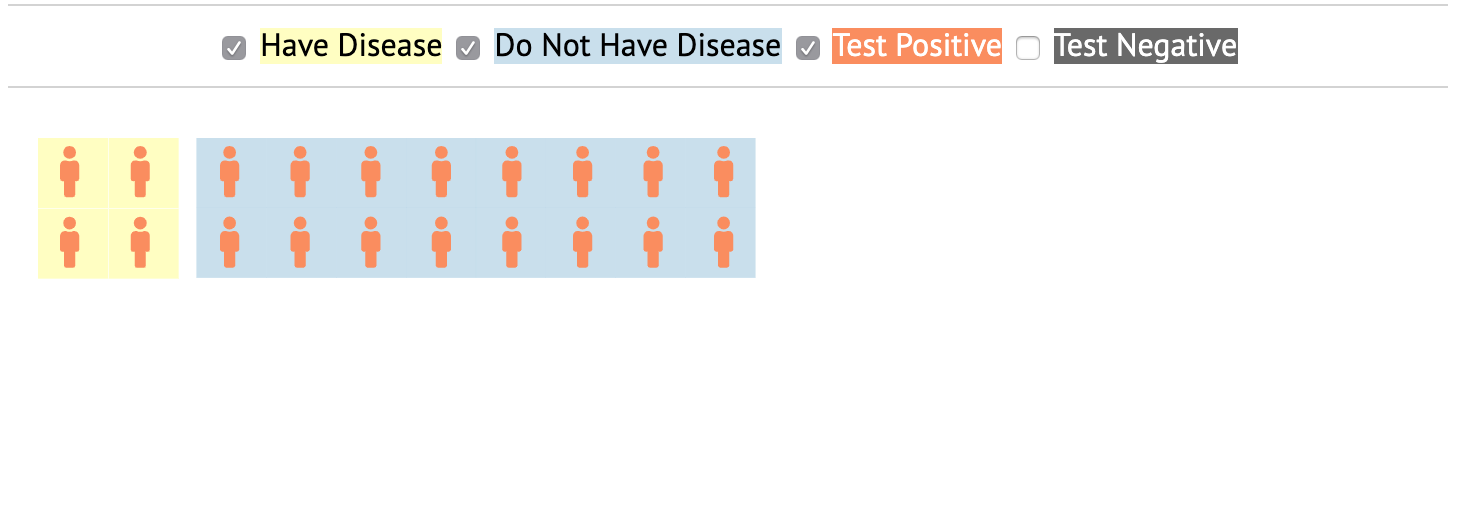
\includegraphics[width=.29\linewidth]{grouped_i.png}
    & 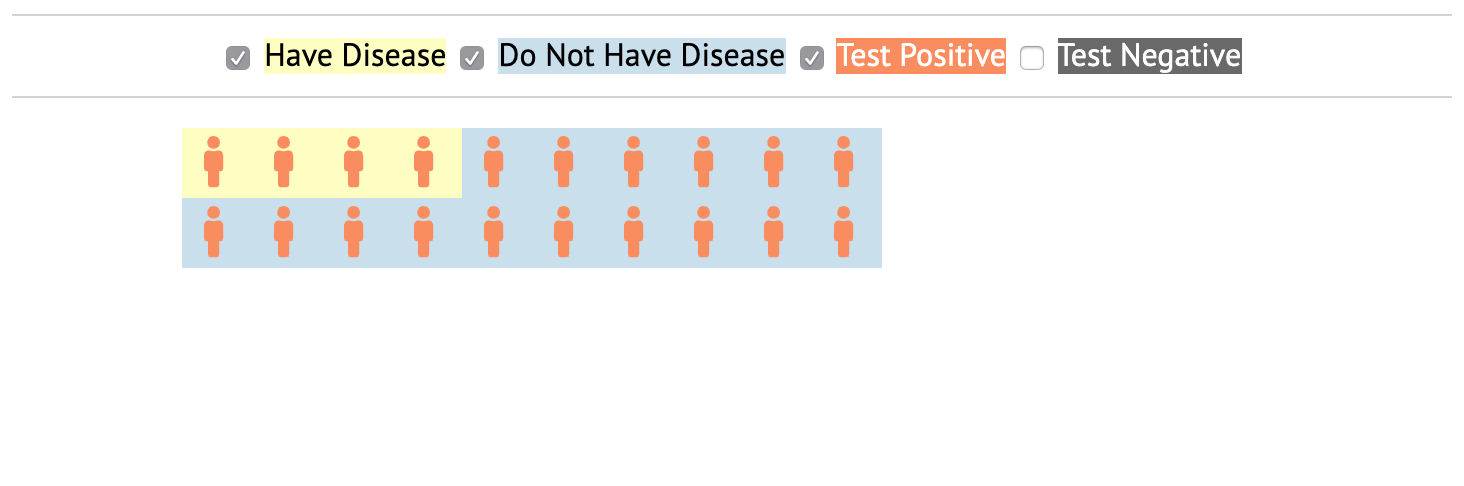
\includegraphics[width=.29\linewidth]{aligned_i.png}  
    & 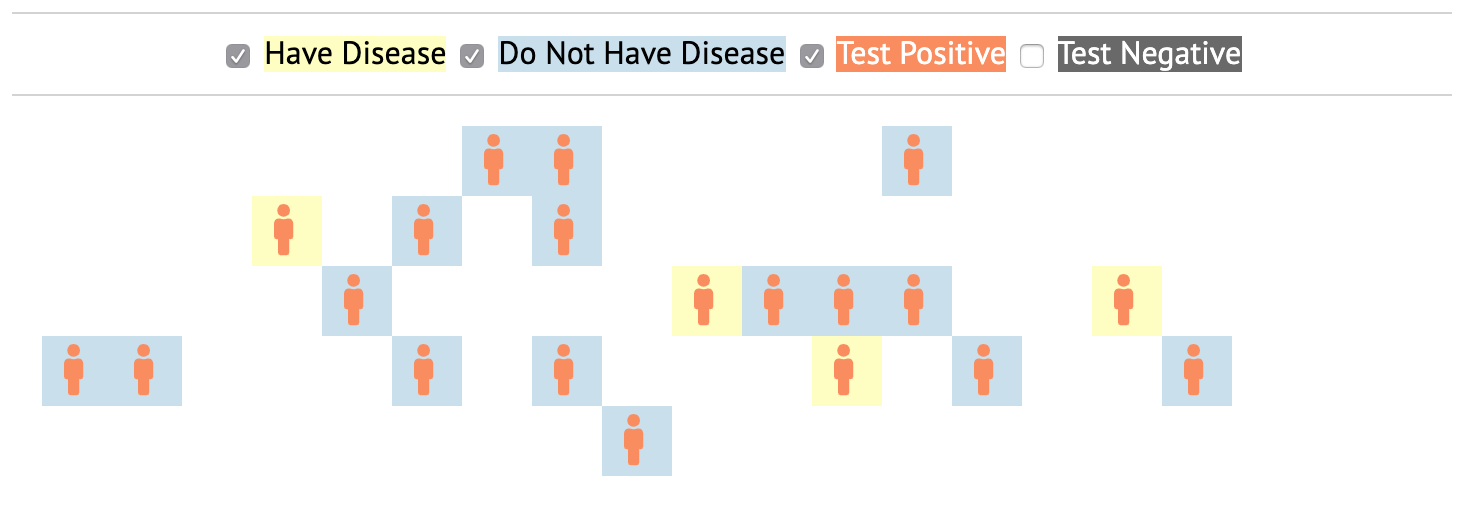
\includegraphics[width=.29\linewidth]{randomized_i.png}
    \\ 
    & \rotatebox{90}{\textit{static}}
    & 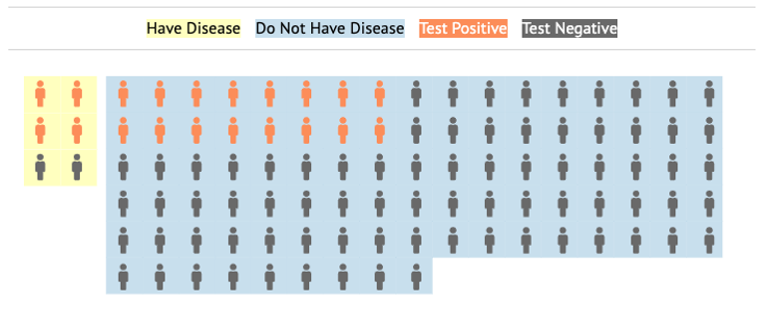
\includegraphics[width=.29\linewidth]{grouped_s.png}
    & 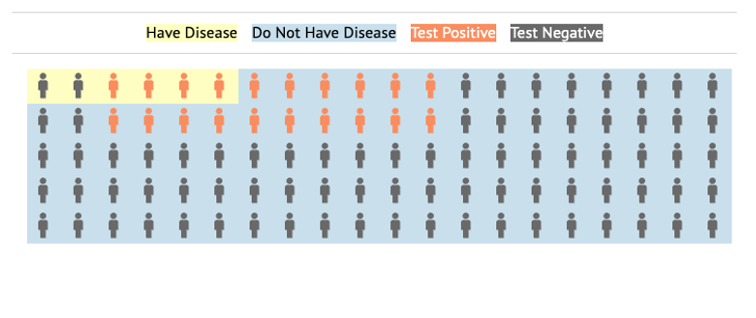
\includegraphics[width=.29\linewidth]{aligned_s.png}  
    & 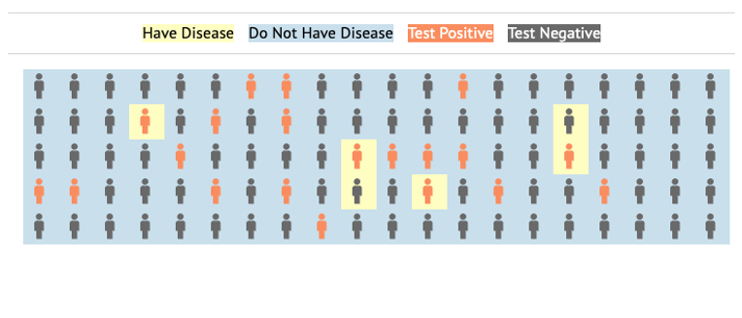
\includegraphics[width=.29\linewidth]{randomized_s.png}
\end{tabular}
\caption{Three interactive and static conditions used in Experiment 1. Full size images are available in supplementary materials.} %\remco{I'm annoyed by the vertical alignment. But after spending two hours digging to latex, I give up! I truly hate latex tables...}}
\label{tab:tabPilotVis}
\end{table*}
\section{Research Goals}
Given the conflicting prior results on how interaction impacts Bayesian reasoning visualizations, the overarching goal of this paper is to empirically test whether adding interaction to a static visualization (i.e. a visualization with no occluded or hidden data that does not require interaction for data exploration) can improve performance on a Bayesian reasoning task. We hypothesize that the mixed results of prior work are partially due to confounding factors between experiments, such as underlying visualization designs and users' spatial ability. %Additionally, prior research has shown that spatial ability plays a strong role in a person's ability to use a visualization, and more specifically, in accuracy on Bayesian reasoning tasks~\cite{liu2020Survey, ottley2016Bayesian}. Thus, we postulate that the effectiveness of interaction also depends on a user's spatial ability. 

The following research questions guide our investigation:
\begin{compacthang}
	\item \textbf{RQ1}: Does adding interaction to a static visualization improve accuracy on a Bayesian reasoning task? 
	\item \textbf{RQ2}: Is the effect of interaction modulated by the effectiveness of the underlying static visualization? 
	\item \textbf{RQ3}: Does users' spatial ability moderate performance on a Bayesian reasoning task with an interactive visualization?   
\end{compacthang}

%We present the results to a crowdsourced study. For the study we design three static (or base) visualizations based on varying theories for visualizing a Bayesian reasoning problem. Using work by Tsai et al.~\cite{tsai2011Interactive} (which found users given interactive Bayesian reasoning visualizations outperformed those given probabilistic Bayesian reasoning text on a Bayesian reasoning task) as a starting point, we add interaction to each base visualization through checkboxes. The checkboxes allow users to hide and un-hide key pieces of the visualization. We compare participants' accuracy with the interactive checkbox visualizations to accuracy with static visualizations, and expect participants assigned the interactive visualization will perform the Bayesian reasoning task with higher accuracy than participants assigned the static visualization. However, we expect base visualization design and users' spatial ability to moderate performance gains. This experiment is a step towards a deeper understanding of interaction in visualization. By empirically demonstrating what specific factors lead to performance gains and losses when making a static visualization interactive, we hope to lay the ground work for better interactive visualization design with evidence-based design guidelines. 

We present the results to a crowdsourced study. For the study we design three static (or base) visualizations based on varying theories for visualizing a Bayesian reasoning problem. We add interaction to each base visualization through checkboxes and compare participants' accuracy with the interactive checkbox visualizations to accuracy with static visualizations. We expect participants assigned the interactive visualization will perform the Bayesian reasoning task with higher accuracy than participants assigned the static visualization. However, we expect base visualization design and users' spatial ability to moderate performance gains.  
This experiment is a step towards a deeper understanding of interaction in visualization. By empirically demonstrating what specific factors lead to performance gains and losses when making a static visualization interactive, we hope to lay the ground work for better interactive visualization design with evidence-based design guidelines. 

 

\section{Experiment}
%\strikeg{The design space for adding interaction to a Bayesian reasoning visualization is large. Micallef et al.~\cite{micallef2012Assessing}, for example, examined six different representations for communicating Bayesian reasoning} \remco{what do the 6 representations have to do with studying interactions? I get what you mean, but these two sentences don't immediately gel. I suggest to delete}. 
Although interaction is commonly used in data visualization, efforts to define \textit{interactivity} are ongoing~\cite{dimara2020What}. Additionally, there is no consensus on the best visualization for Bayesian reasoning~\cite{micallef2012Assessing, khan2015Benefits, ottley2016Bayesian}. As a result, the design space for interactive Bayesian reasoning visualizations is large. 
For this experiment, we simplify the visualization design space by focusing on variants of \textit{icon arrays} -- one of the most popular and well-studied visualizations in this context~\cite{micallef2012Assessing,ottley2016Bayesian,ottley2019Curious}. Furthermore, we narrow the interaction design space to a single category. Following prior work that tested an interactive Bayesian visualization~\cite{tsai2011Interactive}, we add \textit{checkboxes} which allow the user to hide or show visual elements, and create a more explicit link between the text and the graphical encodings. In particular, this experiment examinse whether adding interactive \textit{checkboxes} to a static visualization (\textit{icon array}) improves accuracy in a Bayesian reasoning task, and whether the underlying static visualization (variations of \textit{icon array}) and users' spatial ability modulate the effectiveness of the interaction. %

\subsection{Visualization Designs}
We present users with a Bayesian reasoning problem concerning a disease in the population and the false positive and negative rates associated with testing for the disease (similar to Ottley et al.~\cite{ottley2016Bayesian}). Each stimulus is an icon array that encodes the four key sub-populations of the problem: \textsc{Have Disease}, \textsc{Do Not Have Disease}, \textsc{Test Positive}, and \textsc{Test Negative}. 
Examples of interactive and static stimuli are shown in Table \ref{tab:tabPilotVis}. Below, we describe each experimental factor: 

\begin{itemize}
    \item \textbf{base visualization}: \{ \textit{grouped}, \textit{aligned}, \textit{randomized}  \}
    \item \textbf{interaction}: \{ \textit{interactive (cbAll)}, \textit{static} \}
\end{itemize}


\subsubsection{Base Visualizations}

We observe three primary designs of icon arrays in the literature which were loosely based on theories for how to facilitate Bayesian reasoning. For example, some researchers propose that representing randomness can more accurately communicate the inherent uncertainly in the problem space~\cite{han2011Representing}. Others hypothesize that spatially grouping visual elements aids reasoning~\cite{micallef2012Assessing}. Based on these theories, we design three variations for \textit{icon arrays} by changing the types of contextual placements of icons (see examples in Table~\ref{tab:pilotDemo}).  
Following guidelines of Bertin\cite{bertin}, background color was used to differentiate between members of the population who \textsc{Have Disease} versus \textsc{Do Not Have Disease}, and icon color was used to differentiate between members of the population who \textsc{Test Positive} versus \textsc{Test Negative}. The base visualizations differed in their use of Gestalt principles~\cite{gestalt} to perceptually group the sub-populations of interest in the Bayesian reasoning problem. Specifically, Gestalt principles guided the design of each base visualization as follows: 

\begin{compacthang}
	\item \textit{Grouped: }We use spatial grouping to show the sub-populations and the relationship between visual elements. The \textit{grouped} icon array shows the \textsc{Have Disease} and \textsc{Do Not Have Disease} sub-populations into two separate grids of icons. Additionally, the \textsc{Test Positive} sub-population is in a block aligned at the top left of the visualization. This design is similar to the hybrid Euler-frequency grid diagram used by Micallef et al.\cite{micallef2012Assessing}. 
	
	\item \textit{Aligned: }The \textit{aligned} icon array shows all icons in one 5 X 20 grid. It aligns the sub-population \textsc{Have Disease} in a block at the top left of the grid, and the sub-population \textsc{Test Positive} in a block at the top middle of the grid. A similar design was used by Brase et al.~\cite{brase2009Pictorial}, and Ottley et al.~\cite{ottley2016Bayesian,ottley2019Curious}.
	
	\item \textit{Randomized: }The \textit{randomized} icon array does not spatially group any sub-populations; icons representing members of each of the four  sub-populations are randomly distributed in a 5 X 20 grid. Similar designs are used in medical risk communication by Han et al.~\cite{han2011Representing}.
\end{compacthang}


\subsubsection{Adding Interaction}
Interactivity was added via checkboxes (similar to Tsai et al.~\cite{tsai2011Interactive}) that allowed users to show (checked) or not show (unchecked) key sub-populations on the icon array. As a default, all checkboxes were checked, and one of \{\textsc{Have Disease}, \textsc{Do Not Have Disease}\} as well as one of \{\textsc{Test Positive}, \textsc{Test Negative}\} had to be checked for any sub-populations to show on the visualization. We call this interaction technique \textit{cbAll} (which stands for checkbox where all boxes are initially checked). 

\subsection{Task}
\label{sec:questions}

We ran a between-subjects 2 \{\textit{interaction}\} \textsc{x} 3 \{\textit{base visualization}\} factor experiment. The experimental task was to answer a Bayesian reasoning problem given textual and visual representations of the problem. The textual description and question components of each stimulus were consistent with those used by Ottley et al.~\cite{ottley2016Bayesian}.
 
\begin{compacthang}
\item \textit{Textual description}: There is a newly discovered disease, Disease X, which is transmitted by a bacterial infection found in the population. There is a test to detect whether or not a person has the disease, but it is not perfect. Here is some information about the current research on Disease X and efforts to test for the infection that causes it.  
\smallskip 

There is a total of 100 people in the population. Out of the 100 people in the population, 6 people actually have the disease. Out of these 6 people, 4 will receive a positive test result and 2 will receive a negative test result. On the other hand, 94 people do not have the disease (i.e., they are perfectly healthy). Out of these 94 people, 16 will receive a positive test result and 78 will receive a negative test result.  
\item \textit{Questions}: \\
	(a) How many people will test positive? \_ \_ \_ \\
	(b) Of those who test positive, how many will actually have the disease? \_ \_ \_ 
\end{compacthang}

\subsection{Participants}
We recruited 530 participants from Amazon Mechanical Turk. Participation was restricted to workers in the United States with an approval rating of greater than $90$ percent. Participants were paid a base rate of $\$1.80$ for participation plus a bonus of $\$0.10$ for every correct answer. 

Before analysis, participants who skipped entire sections of the experiment or did not follow instructions ($N = 3$), and participants who self-identified as colorblind  ($N = 55$) were dropped from the data set. 
%Because our experiment explicitly focuses on comparing the \textit{use} of an interactive visualization to a static visualization, we dropped participants who saw an interactive stimulus but did not interact with it ($N = 141$). 
This left $N = 472$ participants distributed among stimuli as shown in Table \ref{tab:pilotN}. Demographics of participants are shown in Table \ref{tab:pilotDemo}. 

\subsection{Procedure}
The experiment followed an approved protocol per Tufts University's IRB, and was posted as a HIT on Amazon Mechanical Turk\footnote{Link to experiment: https://valt.cs.tufts.edu/studies/br4/public/.}. Workers who accepted the HIT followed a link to the experiment. After providing informed consent, participants were taken to an instruction page explaining the experiment.
%that they would be asked to look at a text description and static or interactive visualization of a reasoning problem, and then asked to answer several questions based on the information presented. 
This page demonstrated what the legend for a \textit{static} visualization would look like versus the \textit{cbAll} legend. After the instruction page, participants were shown one of the six experimental stimuli. Participants could take as much time with the stimulus as they wanted before clicking a button to view the questions to answer. 
Clicking said button started an experimental timer that ended when participants submitted their answers.
After completing the main task participants were asked to complete a short demographic questionnaire, the paper folding test (VZ-2) from Ekstrom, French, \& Hardon\cite{paperFolding} to measure spatial ability, and to provide any additional feedback they wished. 

\begin{table}[t!]
  \resizebox{\linewidth}{!}{
  \centering
\begin{tabular}{c|ccc|c}
        & grouped & aligned & randomized & interactive or not total \\ \hline
\textit{cbAll}   & 64     & 100     & 82   & 246 \\ \hline
\textit{static}  & 86    & 70    & 70  &  226 \\ \hline
base total & 150 & 170 & 152 & 472
\end{tabular}}
\caption{Sample sizes (N) for each condition.}
\label{tab:pilotN}
\end{table}


%%%%%%%%%%%%%%%%%%%%%%%%%
%%%%%%%%%%%%%%%%%%%%%%%%%
\begin{table}[h!]
\begin{threeparttable}[b]
\begin{tabular}{ll}
\hline
N                                                                                & 331                                                                                                                                                    \\ \hline
Age                                                                              & \begin{tabular}[c]{@{}l@{}}18-24: 6.4\%, 25-39: 64.4\%, 40-49: 17.2\%, \\ 50-59:7.6\%, 60+: 4.4\%\end{tabular}                                     \\ \hline
Gender                                                                           & \begin{tabular}[c]{@{}l@{}}Female: 38.3\%, Male: 61.0\%, \\ Non-Binary: 0.8\%\end{tabular}                                                             \\ \hline
Education                                                                        & \begin{tabular}[c]{@{}l@{}}High School: 28.6\%, Bachelors: 56.6\%, \\ Masters: 10.2\%, PhD: 1.5\%, Other: 3.2\%\end{tabular}                            \\ \hline
\begin{tabular}[c]{@{}l@{}}Expertise with \\ Statistical \\ Visualization\end{tabular}                  & \begin{tabular}[c]{@{}l@{}}Novice: 21.4\%, Low-intermediate: 20.1\%, \\ Intermediate: 32.3\%, \\ High-intermediate: 17.4\%, Expert: 8.5\%\end{tabular} \\ \hline
\begin{tabular}[c]{@{}l@{}}Statistical Training \\ 1 (none) - \\ 5 (highly trained) \end{tabular} & \begin{tabular}[c]{@{}l@{}}1: 32.4\%, 2: 22.5\%, 3: 16.7\%, \\ 4: 15.3\%, 5: 12.5\%\end{tabular}                                                         \\ \hline
\end{tabular}
\end{threeparttable}
\caption{Participant demographics.}
\label{tab:pilotDemo}
\end{table}
          
\subsection{Hypotheses}
Analysis focuses on answering \textbf{RQ1}, \textbf{RQ2}, and \textbf{RQ3}.
Based on prior work we postulate that the interactive \textit{checkbox} visualization will act as an external representation of users' reasoning process, and therefore reduce cognitive load~\cite{liu2010Mental, pohl2012User}. We expect reduced cognitive load to result in higher accuracy on the Bayesian reasoning task (\textbf{RQ1}). Additionally, we anticipate the extent to which icons in the base visualizations are perceptually grouped will affect cognitive load (i.e. the \textit{grouped} and \textit{aligned} base visualizations which leverage Gestalt principles to perceptually group icons should induce less cognitive load than the \textit{randomized} (un-grouped) base visualization). Thus the reduction of cognitive load from adding interaction (and associated performance gains) should be modulated by base visualization (\textbf{RQ2}). Finally, we expect users with low spatial ability will benefit most from the addition of interaction (\textbf{RQ3}). Ottley et al.~\cite{ottley2016Bayesian} showed people with low spatial ability perform very poorly on Bayesian reasoning tasks. We postulate that the additional cognitive offload afforded by interaction will help users with low spatial ability perform Bayesian reasoning more accurately. We propose the following hypotheses:

\begin{compacthang} 
	\item \textbf{H1}: Participants who use an interactive visualization will be more accurate in answering the Bayesian reasoning question than participants who saw a static visualization. 
	\item \textbf{H2}: Differences in accuracy will be modulated by base (\textit{grouped, aligned, randomized}) visualization design. 
	\item \textbf{H3.1}: Participants with high spatial ability who use an interactive visualization will be as accurate in answering the Bayesian reasoning question as participants who saw a static visualization. 
	\item \textbf{H3.2}: Participants with low spatial ability who use an interactive visualization will be more accurate in answering the Bayesian reasoning question than participants who saw a static visualization. 
\end{compacthang}

\subsection{Findings}
To test our hypotheses, we analyze participant's responses to the questions detailed in Section~\ref{sec:questions}. Consistent with prior work\cite{ottley2016Bayesian, ottley2019Curious}, participants were considered correct only if they answered both parts of the two-part question correctly (that is, 20 people will test positive, and of those 4 will actually have the disease). Our analysis script is included in supplemental materials, however under the guidelines of our IRB we cannot release collected data.

\subsubsection{Does adding interaction to a static visualization improve accuracy on Bayesian reasoning task?}
\label{sec:exp1_analysis}

Figure \ref{fig:exp1_static_vs_int} shows overall the proportion of correct answers for the \textit{interactive} and \textit{static} conditions. We observe that $53\%$ of the participants in the \textit{cbAll} condition entered the correct answers, whereas the \textit{static} visualization had a $57\%$ correct response rate.
We perform a Chi-squared test of $accuracy \sim interactive\_or\_static$, and find no statistically significant difference in accuracy between participants using the \textit{cbAll} versus the \textit{static} visualization ($\chi^2(1, N = 472) = 0.85, p = 0.34$). This suggests that \textit{interaction does not improve reasoning on a Bayesian reasoning task} thus we \textbf{reject H1}.    

\begin{figure}[h!]
    \centering
    \scalebox{0.7}{
    \begin{bchart}[step=.25,max=1,width=\linewidth]
    \bcbar[label=\textit{cbAll}, color=bar-blue]{.53}
    \bcskip{3pt}
    \bcbar[label=\textit{static}, color=bar-blue]{.57}
    \bcxlabel{Proportion of Correct Answers}
    \end{bchart}}
    \caption{Proportion of participants answering the Bayesian reasoning task correctly given an interactive (\textit{cbAll}) versus \textit{static} visualization.}
    \label{fig:exp1_static_vs_int}
\end{figure}

Next, we look at how many participants in the \textit{cbAll} condition actually interacted with the visualization they saw. Out of the $246$ participants assigned to \textit{cbAll}, only $43\%$ used the checkboxes on the visualization. Seventy percent of the participants who interacted with the visualization answered correctly, while only $40\%$ of those who did not interact answered correctly, as shown in Figure \ref{fig:exp1_interacted_vs_did_not}.

We perform a Chi-squared test of $accuracy \sim interacted\_or\_not$, and find a statistically significant difference in accuracy between participants who did and did not interact with the \textit{cbAll} visualization ($\chi^2(1, N = 246) = 22.85, p < 0.001$). Additionally, a Kruskal-Wallis\footnote{We performed a Kruskal-Wallis test because the Shapiro-Wilk Normality test showed this distribution of completion time differed significantly from normal ($W = 0.25, p < 0.01$).} test showed a small significant difference in completion time between participants who did and did not interact ($H(1) = 3.81, p = 0.05$). Overall, participants who did interact completed the task faster than those who did not interact (interacted: $\mu = 47.5s$, $\sigma = 31.0s$; did not interact: $\mu = 52.6s$, $\sigma = 115.2s$). 

\begin{figure}[h!]
    \centering
    \scalebox{0.7}{
    \begin{bchart}[step=.25,max=1,width=\linewidth]
    \bcbar[label=\textit{Interacted}, color=bar-blue]{.70}
    \bcskip{3pt}
    \bcbar[label=\textit{Did Not Interact}, color=bar-blue]{.40}
    \bcxlabel{Proportion of Correct Answers}
    \end{bchart}}
    \caption{Proportion of participants assigned to \textit{cbAll} answering the Bayesian reasoning task correctly grouped by if they interacted or not.}
    \label{fig:exp1_interacted_vs_did_not}
\end{figure}

%retain all participants even those who did not interact 
It is impossible to be certain if participants in the \textit{cbAll} condition who did not interact were simply negligent participants, or if there is some other factor at play. We could drop participants assigned to \textit{cbAll} who did not interact from our analysis in order to specifically compare Bayesian reasoning \textit{using} an interactive visualization to Bayesian reasoning with a static visualization, however this would likely bias the interactive condition to include only very diligent participants, while the static condition would be a mix of diligent and non-diligent workers. Therefore, we continue our analysis without dropping any participants assigned \textit{cbAll} who did not interact. 

\subsubsection{Is the effect of interaction modulated by the underlying static visualization design?}

To investigate whether base visualization had an effect on participants' accuracy independently of interaction we perform a Chi-squared test of $accuracy \sim base\_visualization$. We find no significant difference in accuracy by base ($\chi^2(2, N = 472) = 2.15, p = 0.34$). As shown in Figure~\ref{fig:exp1_bases}, we observe near-equal proportions of correct answers for the three base representations, suggesting that the \textit{variations in the design of icon arrays had no significant effect on accuracy.}

\begin{figure}[h!]
    \centering
    \scalebox{0.7}{
    \begin{bchart}[step=.25,max=1,width=\linewidth]
    \bcbar[label=\textit{grouped}, color=bar-blue]{.57}
    \bcskip{3pt}
    \bcbar[label=\textit{aligned}, color=bar-blue]{.57}
    \bcskip{3pt}
    \bcbar[label=\textit{randomized}, color=bar-blue]{.50}
    \bcxlabel{Proportion of Correct Answers}
    \end{bchart}}
    \caption{Proportion of participants answering the Bayesian reasoning task correctly by base visualization.}
    \label{fig:exp1_bases}
\end{figure}

To better understand the nuances of how a base visualization may affect the value-add of interaction we stratify the data by base visualization (\textit{grouped, aligned, randomized}) and perform a Chi-squared test of $accuracy \sim interactive\_or\_static$ within each base. Proportions of correct answers by interactive vs. static and base visualization are shown in Figure \ref{fig:exp1_static_vs_int_by_base}. 

\begin{figure}[h!]
    \centering
    \scalebox{0.7}{
    \begin{bchart}[step=.25,max=1,width=\linewidth]
    \bcbar[text=\textit{cbAll}, color=bar-cball]{.56}
    \bclabel{\textit{grouped}}
    \bcbar[text=\textit{static}, color=bar-static]{.58}
    \bcskip{6pt}
    
    \bcbar[text=\textit{cbAll}, color=bar-cball]{.59}
    \bclabel{\textit{aligned}}
    \bcbar[text=\textit{static}, color=bar-static]{.54}
    \bcskip{6pt}
    
    \bcbar[text=\textit{cbAll}, color=bar-cball]{.42}
    \bclabel{\textit{randomized}}
    \bcbar[text=\textit{static}, color=bar-static]{.59}
    
    \bcxlabel{Proportion of Correct Answers}
    \end{bchart}}
    \caption{Proportion of participants answering the Bayesian reasoning task correctly by interaction and base visualization.} 
    \label{fig:exp1_static_vs_int_by_base}
\end{figure}


We find no statistically significant difference in accuracy between participants assigned \textit{cbAll} versus \textit{static} in the grouped or aligned base visualizations (grouped: $\chi^2(1, N = 150) = 0.05, p = 0.82$; aligned: ($\chi^2(1, N = 170) = 0.37, p = 0.54$)). This suggests that \textit{within the grouped and aligned base visualizations interaction does not improve accuracy on a Bayesian reasoning task}.  

In contrast, we find a statistically significant difference in accuracy between participants assigned \textit{cbAll} versus \textit{static} in the randomized base visualization ($\chi^2(1, N = 152) = 3.81, p = 0.05$). Interestingly, the proportion of participants who were correct using the \textit{cbAll} visualization is less than that for participants using the \textit{static} visualization (Figure \ref{fig:exp1_static_vs_int_by_base}). This suggests that \textit{within the randomized base visualization interaction significantly decreases accuracy on a Bayesian reasoning task}. 

\medskip 
These stratified analyses suggest that \textit{the value-add of interaction is modulated by base visualization design}, thus we \textbf{accept H2}.   

\subsubsection{Does the effect of interaction change based on a user's spatial ability?}
To identify participants with high versus low spatial ability we split our data across median spatial ability ($5.75$), similar to~\cite{ottley2016Bayesian}. We perform a Chi-squared test of $accuracy \sim interactive\_or\_static$ within each spatial ability group. Figure \ref{fig:exp2_sa_by_interaction} shows proportions of correct answers by interactive or static and participants' spatial ability.  

%\paragraph{High Spatial Ability}
Within both spatial ability groups we find no statistically significant difference in accuracy between participants assigned the \textit{cbAll} visualization and the \textit{static} visualization (high spatial ability: ($\chi^2(1, N =  239) = 1.81, p = 0.18$), low spatial ability: ($\chi^2(1, N =  233) = 0.01, p = 0.93$)). This suggests that \textit{for people with high and low spatial ability interaction does not significantly affect accuracy on Bayesian inference}. 

%\paragraph{Low Spatial Ability}
%Within the low spatial ability group we find no statistically significant difference in accuracy between participants assigned the \textit{cbAll} visualization and the \textit{static} visualization ($\chi^2(1, N =  233) = 0.01, p = 0.93$), suggesting that \textit{for people with low spatial ability interaction does not affect accuracy on Bayesian inference}. 

\begin{figure}[h!]
    \centering
    \scalebox{0.7}{
    \begin{bchart}[step=.25,max=1,width=\linewidth]
    
    \bcbar[text=\textit{High SA},   color=bar-highsa]{.73}
    \bclabel{\textit{cbAll}}
    \bcbar[text=\textit{Low SA},   color=bar-lowsa]{.33}
    \bcskip{6pt}
    
    \bcbar[text=\textit{High SA},   color=bar-highsa]{.80}
    \bclabel{\textit{static}}
    \bcbar[text=\textit{Low SA},   color=bar-lowsa]{.33}
    
    \bcxlabel{Proportion of Correct Answers}
    \end{bchart}}
    \caption{Portion of participants answering the Bayesian reasoning task correctly by spatial ability (SA) and \textit{cbAll} or \textit{static} visualization. } 
    \label{fig:exp2_sa_by_interaction}
\end{figure}

\subsubsection{Does underlying static visualization design moderate the effect of interaction techniques within spatial ability groups?}

Within each spatial ability group we compare participants' accuracy across bases with a Chi-squared test of $accuracy \sim base\_visualization$. Figure \ref{fig:exp2_bases_by_sa} shows proportions of correct answers for each base visualization by participants' spatial ability. Within both groups we find no significant difference in accuracy by base (high spatial ability: ($\chi^2(2, N = 239) = 2.45, p = 0.29$), low spatial ability: ($\chi^2(2, N = 233) = 5.40, p = 0.07$)), suggesting that \textit{for people with high and low spatial ability, performance on a Bayesian reasoning task is not affected by design of the underlying static visualization}. 

\begin{figure}[h]
    \centering
    \scalebox{0.7}{
    \begin{bchart}[step=.25,max=1,width=\linewidth]
    
    \bcbar[text=\textit{High SA},   color=bar-highsa]{.82}
    \bclabel{\textit{grouped}}
    \bcbar[text=\textit{Low SA},   color=bar-lowsa]{.37}
    \bcskip{6pt}
    
    \bcbar[text=\textit{High SA},   color=bar-highsa]{.76}
    \bclabel{\textit{aligned}}
    \bcbar[text=\textit{Low SA},   color=bar-lowsa]{.38}
    \bcskip{6pt}
    
    \bcbar[text=\textit{High SA},   color=bar-highsa]{.71}
    \bclabel{\textit{randomized}}
    \bcbar[text=\textit{Low SA},   color=bar-lowsa]{.22}

    \bcxlabel{Proportion of Correct Answers}
    \end{bchart}}
    \caption{Proportion of participants answering the Bayesian reasoning task correctly by base visualization for each spatial ability group.}
    \label{fig:exp2_bases_by_sa}
\end{figure}

To investigate the effect of interaction technique coupled with underlying static visualization design on participants with high and low spatial ability, we stratify the data by spatial ability group (high, low) and base visualization (grouped, aligned, randomized) and perform a Chi-squared test of $accuracy \sim interaction\_technique$.
Proportions of correct answers by interaction technique, base visualization, and spatial ability are shown in Figure \ref{fig:exp2_corr_by_int_base_SA}. 

For participants with high spatial ability assigned to the the \textit{randomized} base we found a significant difference in accuracy between those assigned the \textit{cbAll} and \textit{static} visualizations ($\chi^2(1, N = 87) = 4.26, p < 0.05$). For all other cases, we found no significant difference in participants' accuracy between between the \textit{cbAll} and \textit{static} visualizations (high spatial ability--grouped: ($\chi^2(1, N = 67) = 0.01, p = 0.75$), aligned: ($\chi^2(1, N = 85) = 0.001, p = 0.97$); low spatial ability--grouped: ($\chi^2(1, N = 83) = 0.04, p = 0.84$), aligned: ($\chi^2(1, N = 85) = 0.001, p = 0.98$), randomized:($\chi^2(1, N = 65) = 0.01, p = 0.91$)). 


\begin{figure}[h!]
    \begin{subfigure}[t]{0.52\columnwidth}
    \scalebox{0.7}{
    \begin{bchart}[step=.25,max=1,width=\linewidth]
    \bcbar[text=\textit{cbAll},  color=bar-cball]{.38}
    \bclabel{\textit{grouped}}
    \bcbar[text=\textit{static},  color=bar-static]{.36}
    \bcskip{6pt}
    
    \bcbar[text=\textit{cbAll},  color=bar-cball]{.38}
    \bclabel{\textit{aligned}}
    \bcbar[text=\textit{static},  color=bar-static]{.38}
    \bcskip{6pt}
    
    \bcbar[text=\textit{cbAll},  color=bar-cball]{.21}
    \bclabel{\textit{randomized}}
    \bcbar[text=\textit{static},  color=bar-static]{.22}
    
    \bcxlabel{Proportion of Correct Answers}
    \end{bchart}}
    \caption{\textbf{Low spatial ability}}
    \label{fig:exp2_corr_by_int_base_SA_low}
    \end{subfigure}%
    ~ 
    \begin{subfigure}[t]{0.48\columnwidth}
    \scalebox{0.7}{
    \begin{bchart}[step=.25,max=1,width=\linewidth]
    \bcbar[text=\textit{cbAll},  color=bar-cball]{.84}
    \bcbar[text=\textit{static},  color=bar-static]{.81}
    \bcskip{6pt}
    
    \bcbar[text=\textit{cbAll},  color=bar-cball]{.76}
    \bcbar[text=\textit{static},  color=bar-static]{.77}
    \bcskip{6pt}
    
    \bcbar[text=\textit{cbAll},  color=bar-cball]{.61}
    \bcbar[text=\textit{static},  color=bar-static]{.81}
    
    \bcxlabel{Proportion of Correct Answers}
    \end{bchart}}
    \caption{\textbf{High spatial ability}}
    \label{fig:exp2_corr_by_int_base_SA_high}
    \end{subfigure}
    \caption{Portion of participants in each spatial ability group answering the Bayesian reasoning task correctly given \textit{cbAll} or \textit{static} and base visualization.}
    \label{fig:exp2_corr_by_int_base_SA}
\end{figure}     

These stratified results suggest that \textit{in certain cases adding interaction to a static visualization can detrimentally effect Bayesian reasoning for people with high spatial ability}, thus we \textbf{reject H3.1}. They also suggest that \textit{for people with low spatial ability performance on a Bayesian reasoning task is not affected by interaction}, thus we \textbf{reject H3.2}. 


%\begin{table*}[t!]
\begin{center}
\begin{tabular}{ccccc}
 &  & \multicolumn{3}{c}{\textsc{Base Visualization}} \\
 &  & \textit{grouped} & \textit{aligned} & \textit{randomized} \\
\multirow{4}{*}{\rotatebox{90}{\textsc{Interaction}}} 
    & \rotatebox{90}{\textit{cbAll} \textbackslash \textit{cbNone}} 
    & 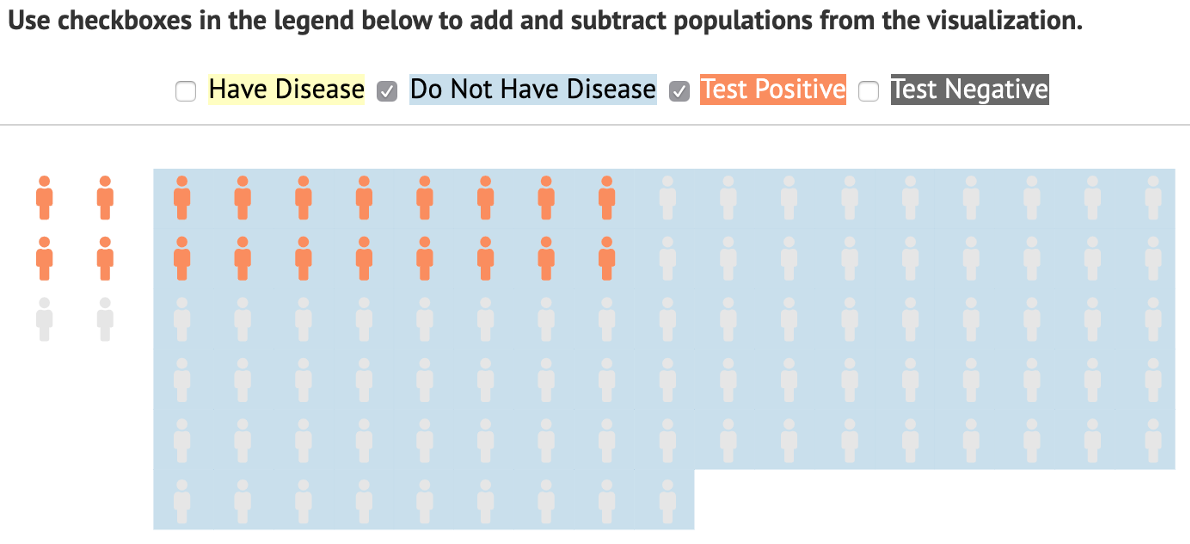
\includegraphics[width=.29\linewidth]{grouped_cbAll.png}  
    & 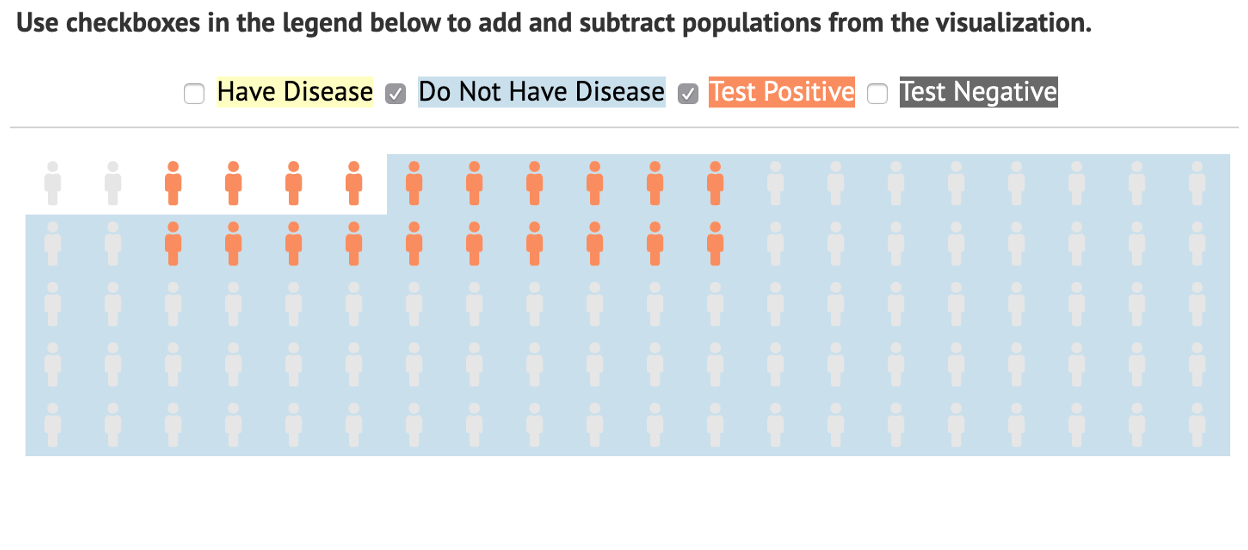
\includegraphics[width=.29\linewidth]{aligned_cbAll.png}  
    & 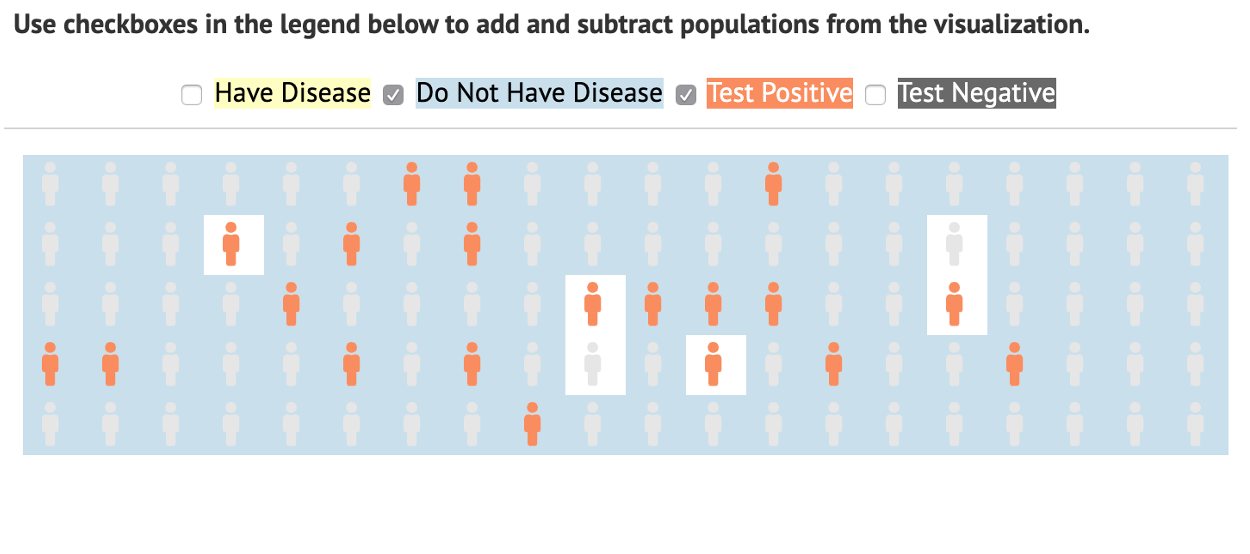
\includegraphics[width=.29\linewidth]{randomized_cbAll.png}
   % \\
   % & \rotatebox{90}{\textit{cbNone}} 
   % & 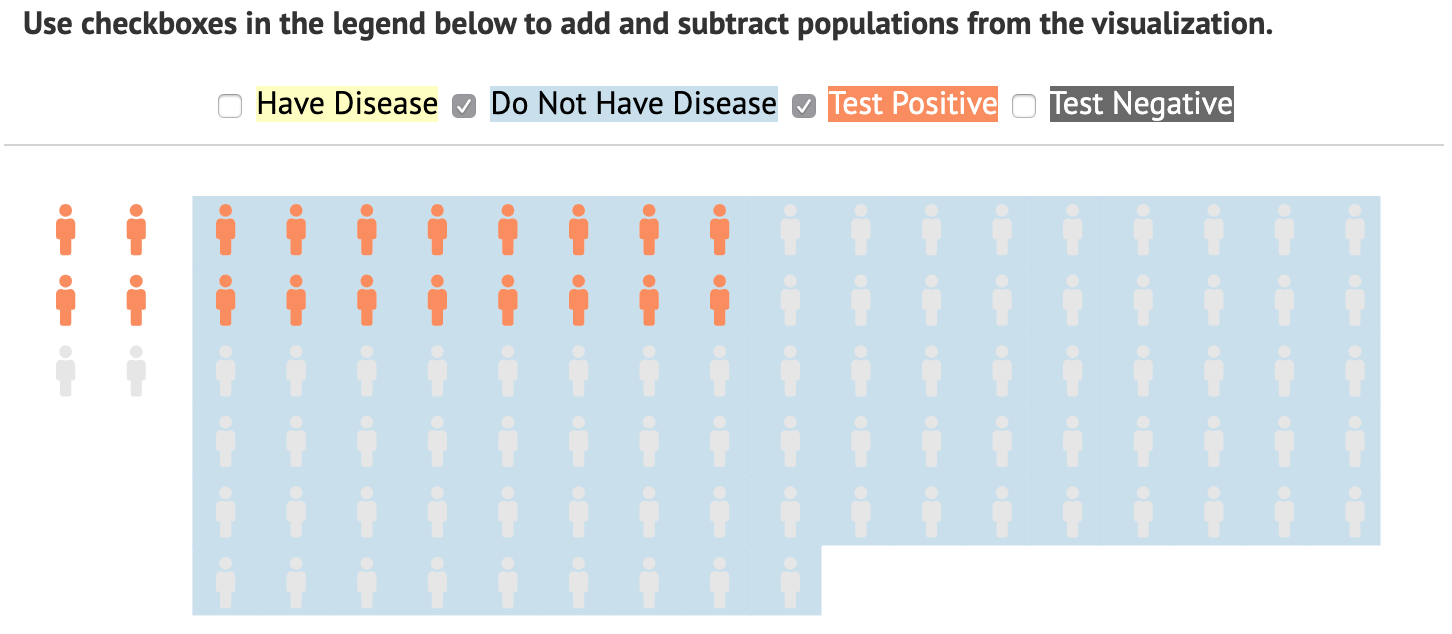
\includegraphics[width=.29\linewidth]{grouped_cbNone.png}  
   % & 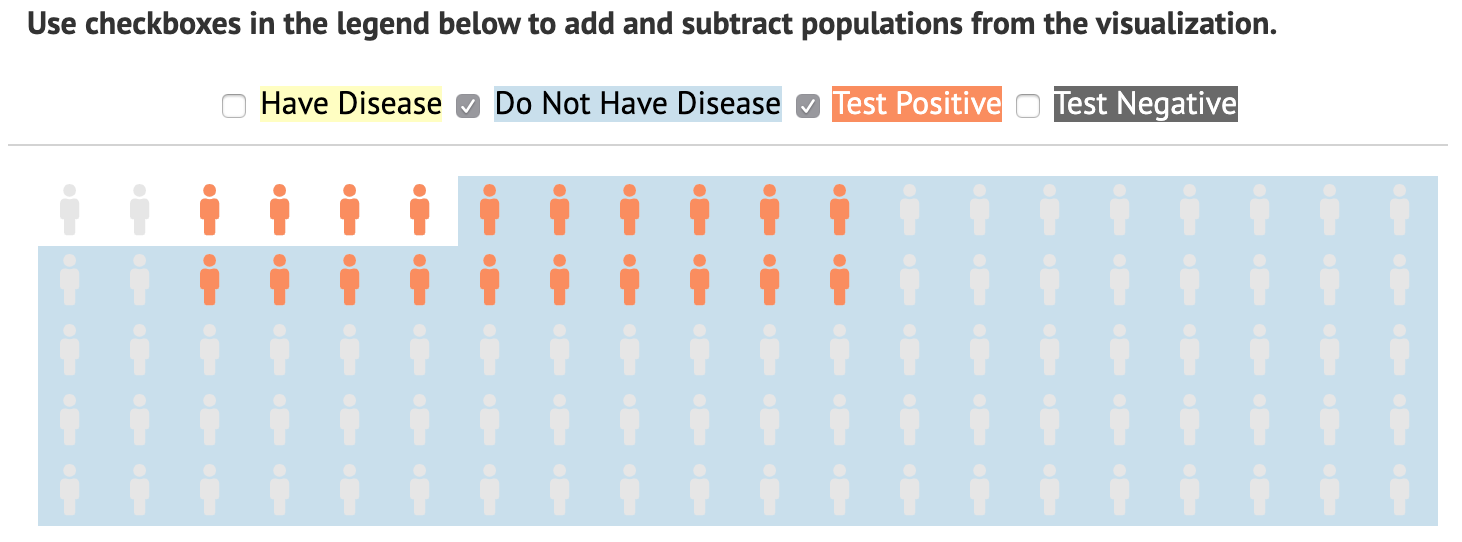
\includegraphics[width=.29\linewidth]{aligned_cbNone.png}  
   % & 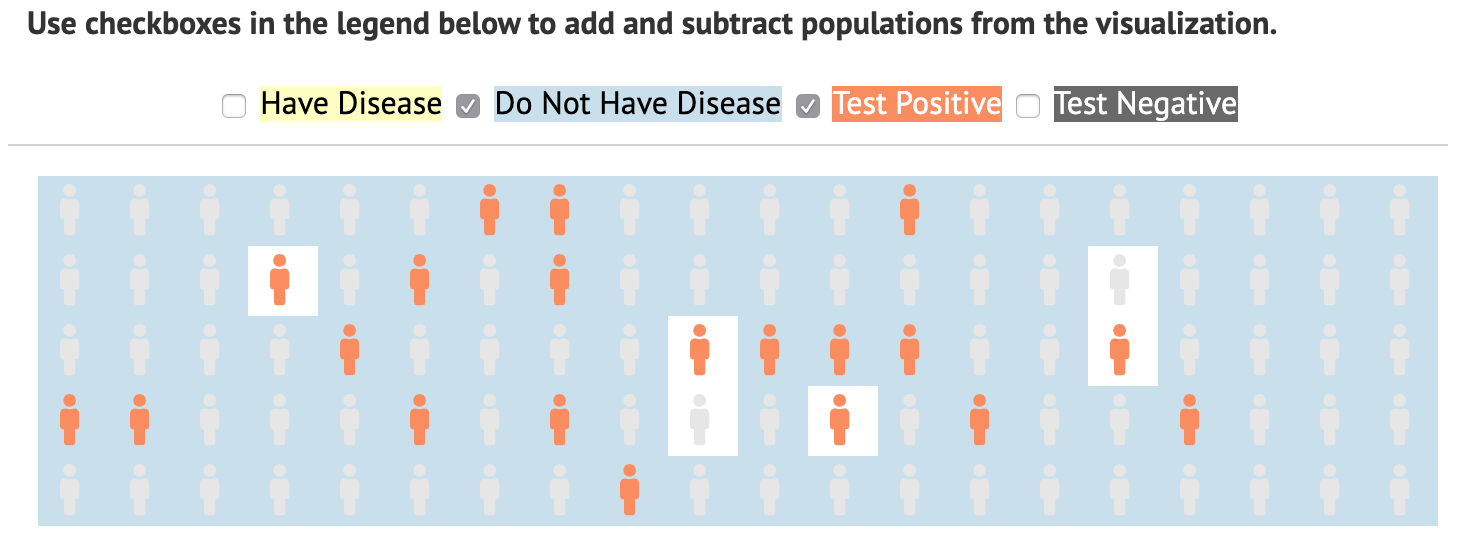
\includegraphics[width=.29\linewidth]{randomized_cbNone.png}
    \\
    & \rotatebox{90}{\textit{drag}} 
    & 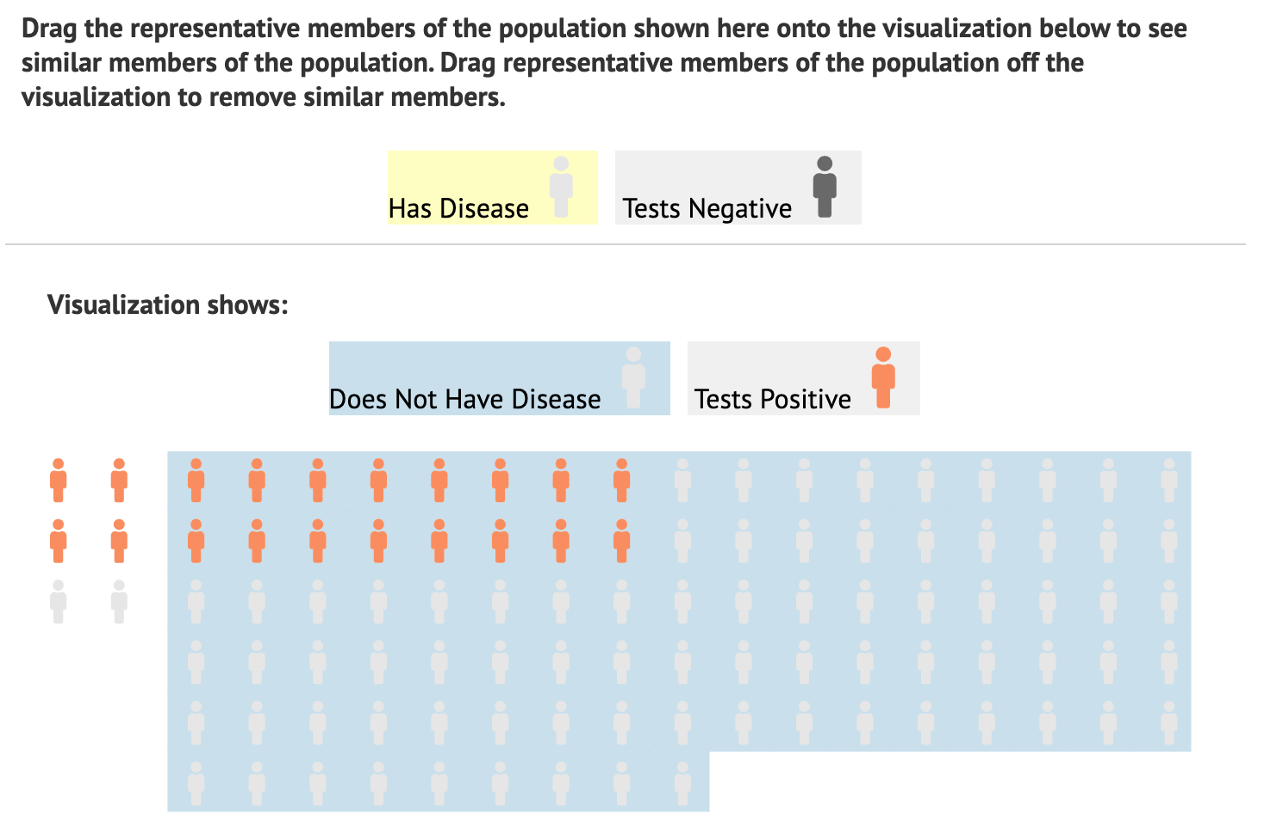
\includegraphics[width=.29\linewidth]{grouped_drag.png}  
    & 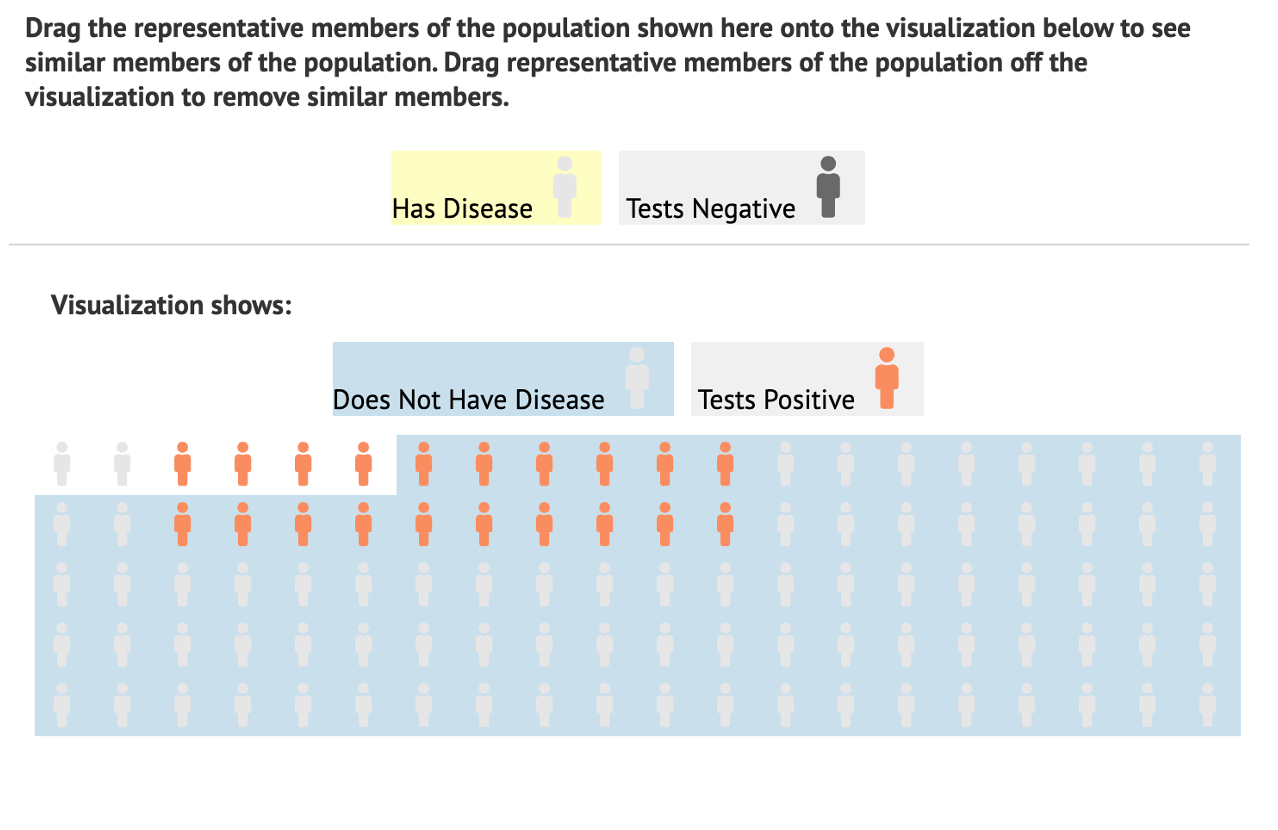
\includegraphics[width=.29\linewidth]{aligned_drag.png}  
    & 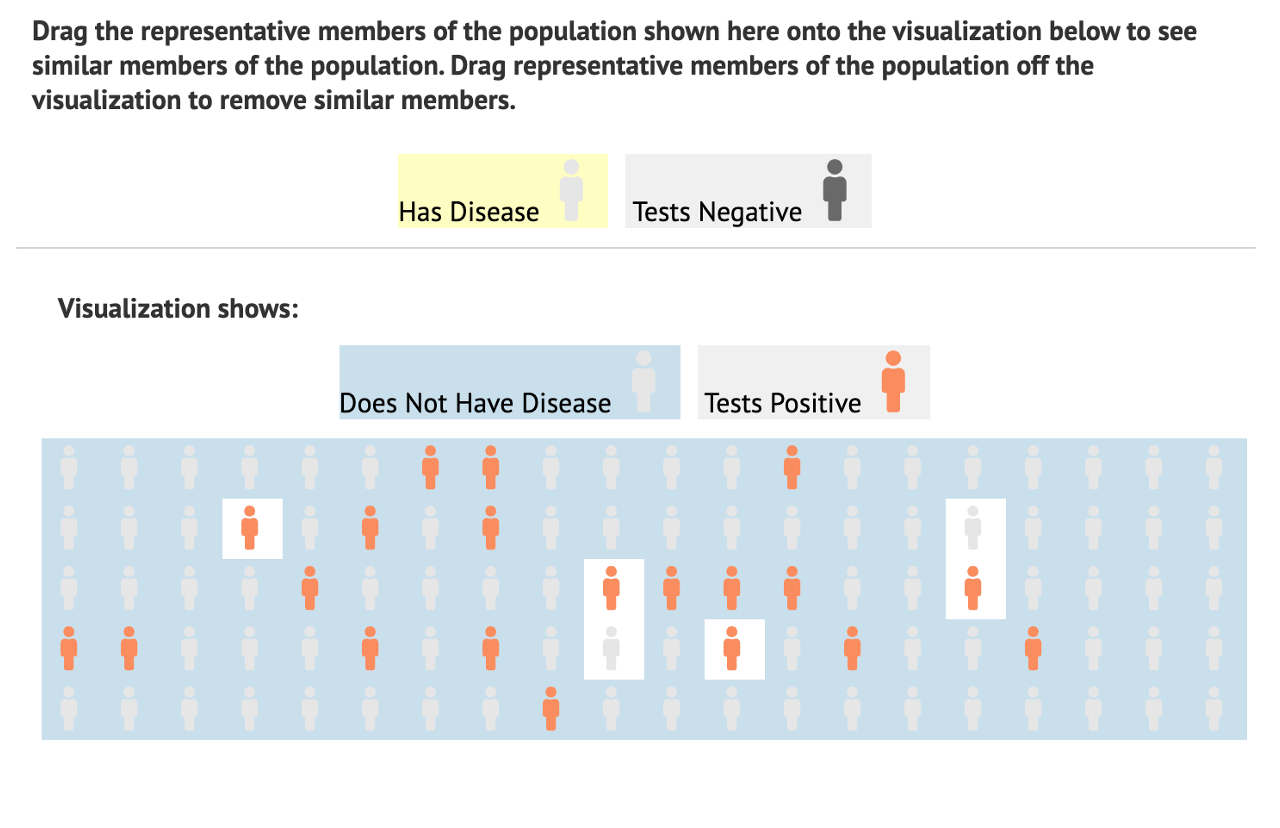
\includegraphics[width=.29\linewidth]{randomized_drag.png}
    \\
    & \rotatebox{90}{\textit{hover}} 
    & 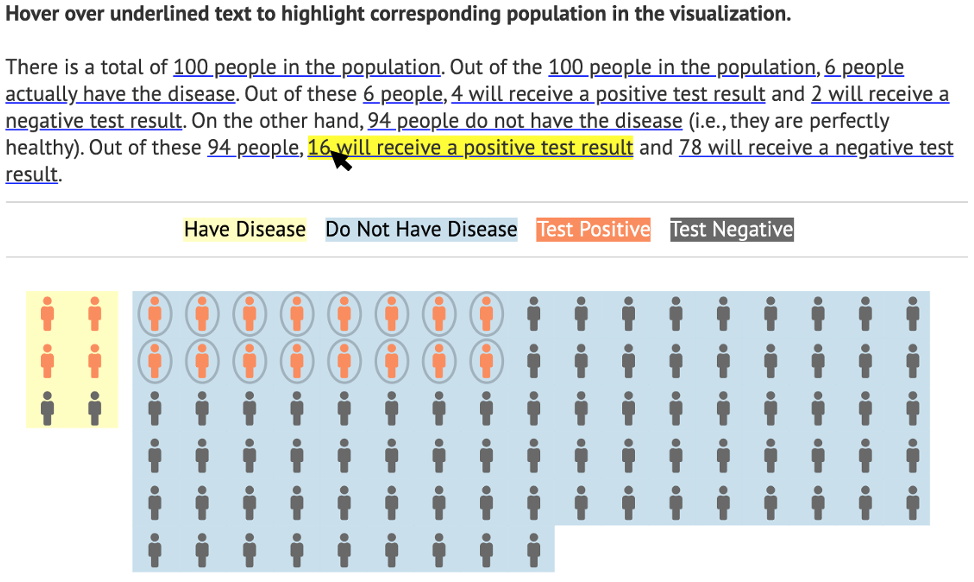
\includegraphics[width=.29\linewidth]{grouped_hover.png}  
    & 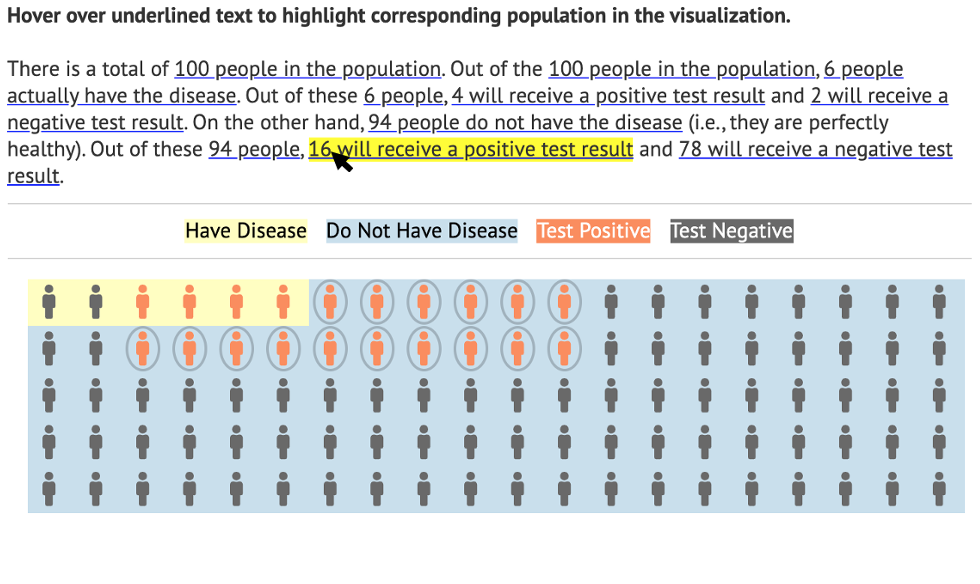
\includegraphics[width=.29\linewidth]{aligned_hover.png}  
    & 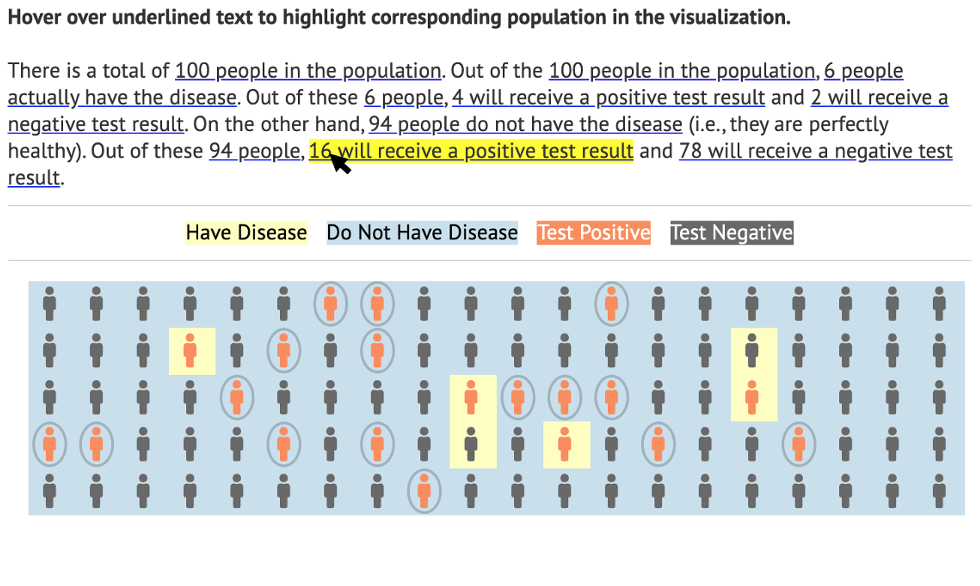
\includegraphics[width=.29\linewidth]{randomized_hover.png}
    \\
    & \rotatebox{90}{\textit{tooltip}} 
    & 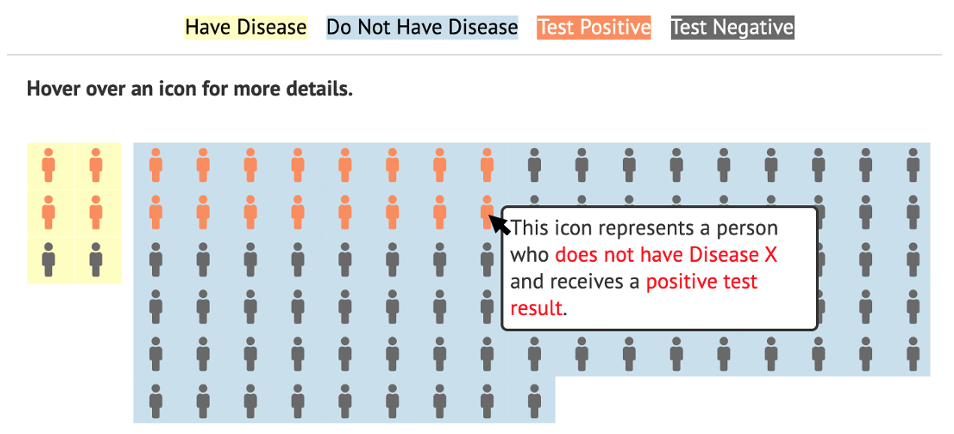
\includegraphics[width=.29\linewidth]{grouped_tooltip.png}  
    & 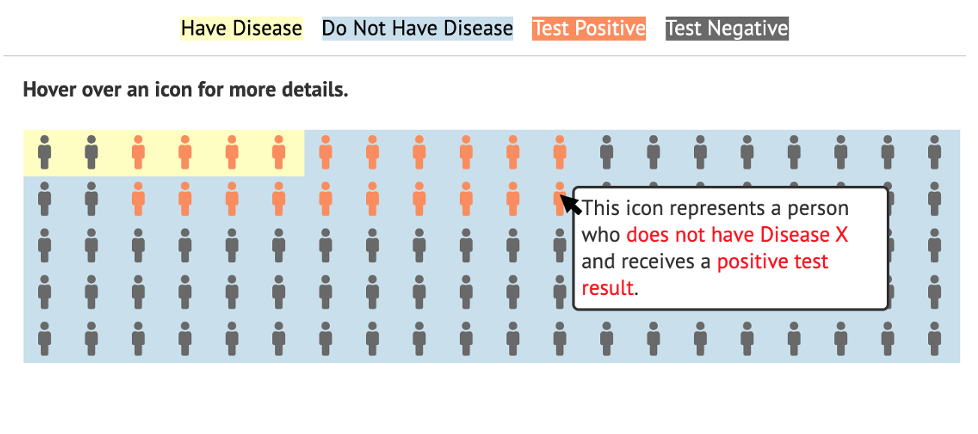
\includegraphics[width=.29\linewidth]{aligned_tooltip.png}  
    & 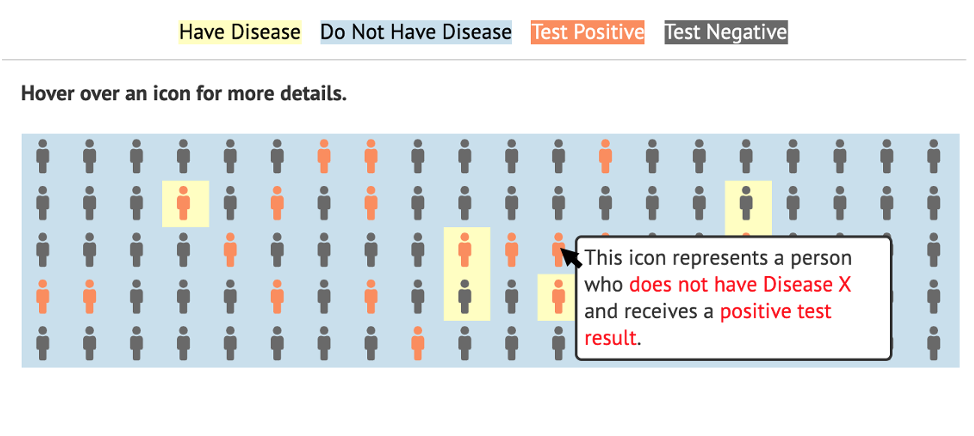
\includegraphics[width=.29\linewidth]{randomized_tooltip.png}
\end{tabular}
\end{center}
\caption{Five interactive conditions used in Experiment 2. Full size images are available in supplementary materials.}
\label{tab:tabFullVis}
\end{table*}


\section{Experiment 2}
The findings of Experiment 1 demonstrated that, depending on the base visualization, adding a \textit{checkbox} interaction to a static Bayesian inference visualization can improve users' reasoning accuracy. Experiment 2 builds on this result by exploring the effect of different interaction designs (\textbf{RQ3}). Specifically, we compare the effects of adding \textit{two types of checkboxes}, \textit{drag and drop}, \textit{brushing and linking}, and \textit{tooltips} to the three \textit{icon array} base visualizations used in Experiment 1. 
In addition to investigating interaction designs, we also examine whether spatial ability moderates the effectiveness of the added interaction (\textbf{RQ4}). Prior work shows that spatial ability plays a significant role in the effective utilization of visualizations~\cite{liu2020Survey}, and in Bayesian reasoning~\cite{ottley2016Bayesian}. Thus we postulate spatial ability can mediate the value-add of interaction to a static Bayesian reasoning visualization. 

\subsection{Visualization Designs}
Consistent with Experiment 1, each stimulus was an icon array that encoded the four key sub-populations in the Bayesian reasoning problem. %: \textsc{Have Disease},  \textsc{Do Not Have Disease}, \textsc{Test Positive}, and  \textsc{Test Negative}. 
Examples of stimuli are shown in Table \ref{tab:tabFullVis}. Experimental factors were:
\begin{itemize}
    \item \textbf{base visualization}: \{\textit{grouped, aligned, randomized}\}
    \item \textbf{interaction technique}: \{\textit{checkboxes (cbAll, cbNone), drag and drop (drag), brushing and linking (hover), tooltips (tooltip)}\}
\end{itemize}

\subsubsection{Base Visualizations}
Experiment 2 used the same three \textit{icon array} base visualizations as Experiment 1 (\textit{grouped}, \textit{aligned}, \textit{randomized}). 

\subsubsection{Interaction Techniques}
We tested five different interaction techniques. Two types of checkboxes were included for consistency with Experiment 1, and because they were tested in prior work on interactive Bayesian reasoning visualizations~\cite{tsai2011Interactive}. Similarly, we included drag and drop as an interaction technique because of its use in prior work on interactive Bayesian reasoning visualizations~\cite{khan2018Interactive}. 
In addition, we tested brushing and linking and tooltips. We included these techniques because they are popular in the visualization community, and are representations of the well known ``\textit{overview first, zoom and filter, details on demand}" mantra of visualization design~\cite{shneiderman1996Eyes}. We chose brushing and linking as an interaction representative of the \textit{zoom and filter} portion of the mantra,
%Moreover, prior work found that people struggle to integrate text and visual representations of the Bayesian reasoning problem\cite{ottley2016Bayesian, ottley2019Curious}. We hypothesize that brushing and linking between text and visualization may overcome this problem. 
and tooltips as an example of the \textit{details on demand} portion of the mantra. Implementation of each technique is explained below:    

\begin{compacthang} 
\item \textbf{\textit{Checkbox All}}: The \textit{cbAll} interaction technique from Experiment 1 was tested in Experiment 2 with a minor modification. Any sub-population checked on the legend is shown on the visualization with color. Any sub-population unchecked on the legend is shown on the visualization with light grey placeholders.      

\item \textbf{\textit{Checkbox None}}: Checkbox None (\textit{cbNone}) is identical to \textit{cbAll}, except all checkboxes are unchecked by default. In other words, the page loads with only light grey placeholders shown on the visualization. 
   
 \item \textbf{\textit{Drag and Drop}}: Drag and drop (\textit{drag}) is a direct manipulation interaction. In practice, \textit{drag} functions identically to \textit{cbNone} expect that participants drag legend labels onto and off of the visualization to show or not show sub-populations.% (as opposed to checking and unchecking checkboxes). 

 \item \textbf{\textit{Brushing and Linking}}:  Brushing and linking (\textit{hover}) is an example of a filter interaction. As participants hover their mouse over areas of text describing sub-populations in the visualization, the text and corresponding sub-population are highlighted. % in the visualization. %\remco{is the reverse true? Does hovering over the visualization highlight text? If so, say that} \ab{no it's not, there is no good mapping in the reverse direction}

\item \textbf{\textit{Tooltip}}: Tooltips (\textit{tooltip}) are an example of details on demand. When a participant hovers their mouse over any icon in the visualization a text box appears describing to which of the four sub-populations that particular icon belongs.  

\end{compacthang}

\subsection{Task}
We ran a between-subjects 5 \{\textit{interaction techniques}\} \textsc{x} 3 \{\textit{base visualizations}\} factor experiment. The same textual description and questions were used as in Experiment 1 (Section \ref{sec:questions}).  

\subsection{Participants}
We recruited 2,149 participants from Amazon Mechanical Turk. Participation was restricted to workers in the United States with an approval rating greater than $90$ percent. Participants were paid a base rate of $\$0.80$ for participation, plus a bonus of $\$0.10$ for every correct answer. 

Before analysis, participants who skipped entire sections of the experiment or did not follow instructions ($N = 35$), participants who self-identified as colorblind ($N = 134$), and participants who saw an interactive visualization but did not interact with it ($N = 473$) were dropped from the data set. 
%\strike{To reiterate, participants who did not interact with a visualization were dropped in order to isolate the effect of \textit{using} interaction from the effect of interaction simply being present in a visualization}.  
There were $N = 1,507$ remaining participants. Demographics of participants are shown in Table \ref{tab:fullDemo}.  

\begin{table}[h!]
\begin{threeparttable}[b]
\begin{tabular}{ll}
\hline
N                                                                                & 1,507                                                                                                                                                    \\ \hline
Age                                                                              & \begin{tabular}[c]{@{}l@{}}18-24: 8.1\%, 25-39: 51.0\%, 40-49: 20.1\%, \\ 50-59: 12.8\%, 60+: 7.7\%\end{tabular}                                     \\ \hline
Gender                                                                           & \begin{tabular}[c]{@{}l@{}}Female: 53.7\%, Male: 45.6\%, \\ Non-Binary: 0.3\%\end{tabular}                                                             \\ \hline
Education                                                                        & \begin{tabular}[c]{@{}l@{}}High School: 28.3\%, Bachelors: 49.1\%, \\ Masters: 14.7\%, PhD: 1.4\%, Other: 5.9\%\end{tabular}                            \\ \hline
\begin{tabular}[c]{@{}l@{}}Expertise with \\ Statistical \\ Visualization\end{tabular}                  & \begin{tabular}[c]{@{}l@{}}Novice: 15.8\%, Low-intermediate: 22.0\%, \\ Intermediate: 38.6\%, \\ High-intermediate: 17.9\%, Expert: 5.0\%\end{tabular} \\ \hline
\begin{tabular}[c]{@{}l@{}}Statistical Training \\ 1 (none) - \\ 5 (highly trained) \end{tabular} & \begin{tabular}[c]{@{}l@{}}1: 30.5\%, 2: 23.6\%, 3: 21.5\%, \\ 4: 15.5\%, 5: 7.4\%\end{tabular}                                                         \\ \hline
\end{tabular}
\end{threeparttable}
\caption{Experiment 2 participant demographics.}
\label{tab:fullDemo}
\end{table}

In order to analyze how the various interaction techniques compared to static we included the \textit{static} group from Experiment 1 as an ``interaction technique" in the analysis of Experiment 2, bringing the total number of participants to $N = 1,733$. From here forward the term ``interaction techniques" refers to \textit{cbAll}, \textit{cbNone}, \textit{drag}, \textit{hover}, \textit{tooltip}, and \textit{static}. Participants were assigned to stimuli as shown in Table \ref{tab:fullN}. 

\begin{table}[h!]
  \resizebox{\linewidth}{!}{
  \centering
\begin{tabular}{c|ccc|c}
        & grouped & aligned & randomized &  interaction technique total\\ \hline
\textit{cbAll}   & 42     & 59     & 64 & 165    \\ \hline
\textit{cbNone}  & 131    & 113    & 117 & 361  \\ \hline
\textit{drag}    & 75     & 79     & 99 &   253  \\ \hline
\textit{hover}   & 109    & 114    & 141 & 364   \\ \hline
\textit{tooltip} & 122    & 132    & 110 & 364 \\ \hline
\textit{static}  & 86    & 70    & 70  &  226 \\ \hline
base total &  565 & 567 & 601 & 1733           
\end{tabular}}
\caption{Sample sizes (N) for each condition in Experiment 2.}
\label{tab:fullN}
\end{table}

\subsection{Procedure}
Experiment 2 followed the same procedure as Experiment 1 with two exceptions. First, there was no instruction page, instead instructions were provided alongside each stimulus. And second, participants were asked to complete a an additional NASA-TLX\cite{NASATLX} survey after the completion of the main study to measure task difficulty.

\subsection{Hypotheses}
Analyses for Experiment 2 focused on answering \textbf{RQ3} and \textbf{RQ4}. We postulate that the conflicting conclusions on whether interactive visualization improves (Tsai et. al~\cite{tsai2011Interactive}) or impedes (Khan et al.~\cite{khan2018Interactive}) Bayesian reasoning may be due to differences in underlying static visualizations, and different interaction designs. Consistent with our findings from Experiment 1, we anticipate that the value-add of interaction will be moderated by base visualization and interaction technique (\textbf{RQ3}). Furthermore, %\replace{it is well established that spatial ability effects visualization usage in general~\cite{liu2020Survey}, and performance on Bayesian inference~\cite{ottley2016Bayesian}. Consistent with prior studies on spatial ability and visualization~\cite{liu2020Survey}, we expect users with high spatial ability to adapt and benefit more from interactivity than users with low spatial ability (\textbf{RQ4})}{
we hypothesize that participants' spatial ability will affect their ability to use the visualization to solve the Bayesian reasoning task. Ottley et al.\cite{ottley2016Bayesian} reported that people with high spatial ability perform Bayesian reasoning significantly better than those with low spatial ability. Additionally, investigations into general visualization usage often show that people with high spatial ability are more adaptable to different visualization designs than people with low spatial ability~\cite{liu2020Survey}. In this experiment, we evaluate whether these trends will hold for the use of interactive Bayesian inference visualizations. Specifically, we propose the following hypotheses:

\begin{compacthang} 
	\item \textbf{H3.1}: Participants' accuracy will differ by interaction technique (\textit{cbAll, cbNone, drag, hover, tooltip, static}). 
	\item \textbf{H3.2}: Participants' accuracy will differ by interaction technique (\textit{cbAll, cbNone, drag, hover, tooltip, static}) and base visualization (\textit{grouped, aligned, randomized}).  
	\item \textbf{H4.1}: Participants with high spatial ability will perform equally well given any interaction technique (\textit{cbAll, cbNone, drag, hover, tooltip, static}). 
	\item \textbf{H4.2}: Participants with low spatial ability will perform differently depending on a visualization's interaction technique (\textit{cbAll, cbNone, drag, hover, tooltip, static}).
	\item \textbf{H4.3}: Participants with high spatial ability will perform equally well given any interaction technique (\textit{cbAll, cbNone, drag, hover, tooltip, static}) and base visualization (\textit{grouped, aligned, randomized}). 
	\item \textbf{H4.4}: Participants with low spatial ability will perform differently depending on a visualization's interaction technique (\textit{cbAll, cbNone, drag, hover, tooltip, static})  and base visualization (\textit{grouped, aligned, randomized}).
	
	%\remco{not sure if we should separate this into 4.1 and 4.2 because these two hypotheses are quite nuanced... Without some explanation and background, it could be hard for a reader to understand why we would hypothesize differently for high SA verus low SA participants}
\end{compacthang}

\subsection{Findings}
For each of these hypotheses we performed chi-squared tests to check for significant differences in proportions of correct answers (accuracy). As with Experiment 1, participants were considered correct only if they answered both parts of the two-part question correctly. 

\begin{figure}[h!]
    \centering
    \scalebox{0.7}{
    \begin{bchart}[step=.25,max=1,width=\linewidth]
    \bcbar[label=\textit{cbAll}, color=bar-blue]{.62}
    \bcskip{3pt}
    \bcbar[label=\textit{cbNone}, color=bar-blue]{.58}
    \bcskip{3pt}
    \bcbar[label=\textit{drag}, color=bar-blue]{.57}
    \bcskip{3pt}
    \bcbar[label=\textit{hover}, color=bar-blue]{.48}
    \bcskip{3pt}
    \bcbar[label=\textit{tooltip}, color=bar-blue]{.53}
    \bcskip{3pt}
    \bcbar[label=\textit{static}, color=bar-blue]{.57}
    \bcxlabel{Proportion of Correct Answers}
    \end{bchart}}
    \caption{Portion of participants answering the Bayesian reasoning task correctly given each interaction technique.} %There is a significant pairwise difference between \textit{cbAll} and \textit{hover} ($\chi^2(1, N = 529) = 8.59, p = 0.003$).}
    \label{fig:exp2_interactions}
\end{figure}

\subsubsection{Do different interaction techniques have different effects on accuracy in Bayesian reasoning?} 
We performed a chi-squared test of $accuracy \sim interaction\_technique$, and found a statistically significant difference in accuracy between participants using different interaction techniques ($\chi^2(5, N = 1733 ) = 12.34, p < 0.05$). Pairwise chi-squared tests of interaction techniques with a Bonferroni corrected alpha ($\alpha=0.003$) showed a significant difference between \textit{cbAll} and \textit{hover} ($\chi^2(1, N = 529) = 8.59, p = 0.003$). As shown in Figure \ref{fig:exp2_interactions}, a higher proportion of participants answered the Bayesian reasoning task correctly with the \textit{cbAll} visualization than with the \textit{hover} visualization. These results suggest that \textit{the design of an interactive technique affects the value-add of interaction}, thus we \textbf{accept H3.1}. % depends on design different interaction techniques 
%\remco{Bonferonni correction is very aggressive / conservative, but it's the right thing to do here. The question is, if space permits, would it make sense to list all the p-values? This could give the reader a sense of what the differences are like without the constraint of a very small alpha.}

\begin{figure}[h!]
    \centering
    \scalebox{0.7}{
    \begin{bchart}[step=.25,max=1,width=\linewidth]
    \bcbar[label=\textit{grouped}, color=bar-blue]{.57}
    \bcskip{3pt}
    \bcbar[label=\textit{aligned}, color=bar-blue]{.56}
    \bcskip{3pt}
    \bcbar[label=\textit{randomized}, color=bar-blue]{.52}
    \bcxlabel{Proportion of Correct Answers}
    \end{bchart}}
    \caption{Portion of participants answering the Bayesian reasoning task correctly by base visualization.}
    \label{fig:exp2_bases}
\end{figure}

\subsubsection{Is the effect of interaction moderated by interaction design and the underlying static visualization design?}
We compared participants' accuracy across base visualizations with a chi-squared test of $accuracy \sim base\_visualization$. We found no significant difference in accuracy by base ($\chi^2(2, N = 1733) = 2.98, p = 0.23$), suggesting that \textit{design of the underlying static visualization has no effect on participants' accuracy in a Bayesian reasoning task}. Figure \ref{fig:exp2_bases} shows proportions of correct answers by base visualization. 

\begin{figure}[h!]
    \centering
    \scalebox{0.7}{
    \begin{bchart}[step=.25,max=1,width=\linewidth]
    \bcbar[text=\textit{cbAll},  color=bar-cball]{.74}
    \bcbar[text=\textit{cbNone}, color=bar-cbnone]{.59}
    \bcbar[text=\textit{drag},   color=bar-drag]{.60}
    \bclabel{\textit{grouped}}
    \bcbar[text=\textit{hover},   color=bar-hover]{.51}
    \bcbar[text=\textit{tooltip}, color=bar-tooltip]{.52}
    \bcbar[text=\textit{static},  color=bar-static]{.58}
    \bcskip{6pt}
    
    \bcbar[text=\textit{cbAll},  color=bar-cball]{.61}
    \bcbar[text=\textit{cbNone}, color=bar-cbnone]{.65}
    \bcbar[text=\textit{drag},   color=bar-drag]{.51}
    \bclabel{\textit{aligned}}
    \bcbar[text=\textit{hover},   color=bar-hover]{.48}
    \bcbar[text=\textit{tooltip}, color=bar-tooltip]{.55}
    \bcbar[text=\textit{static},  color=bar-static]{.54}
    \bcskip{6pt}
    
    \bcbar[text=\textit{cbAll},  color=bar-cball]{.55}
    \bcbar[text=\textit{cbNone}, color=bar-cbnone]{.50}
    \bcbar[text=\textit{drag},   color=bar-drag]{.60}
    \bclabel{\textit{randomized}}
    \bcbar[text=\textit{hover},   color=bar-hover]{.45}
    \bcbar[text=\textit{tooltip}, color=bar-tooltip]{.52}
    \bcbar[text=\textit{static},  color=bar-static]{.59}
    
    \bcxlabel{Proportion of Correct Answers}
    \end{bchart}}
    \caption{Portion of participants answering the Bayesian reasoning task correctly given each interaction technique by base visualization.}
    \label{fig:exp2_interactions_by_base}
\end{figure}

Similar to Experiment 1, we stratified data by base visualization (grouped, aligned, randomized) and performed a chi-squared test of $accuracy \sim interaction\_technique$ within each base. Proportions of correct answers by base visualization and interaction technique are shown in Figure \ref{fig:exp2_interactions_by_base}. We found no significant differences in accuracy between participants assigned different interaction techniques within each base (grouped: ($\chi^2(5, N = 565) = 7.77, p = 0.17$), aligned: ($\chi^2(5, N = 567) = 7.75, p = 0.17$), randomized:($\chi^2(5, N = 601) = 6.42, p = 0.27$)), suggesting that \textit{the combination of interaction technique and underlying base visualization has no effect on participants' accuracy in a Bayesian reasoning task}, and causing us to \textbf{reject H3.2} %\remco{Ahhh, this is so confusing and weird! Is H3 about how how different interaction techniques improve reasoning? Or is it about how different interaction techniques, when used with different visualization types, produce different outcomes?}.


\subsubsection{Does the effect of different interaction techniques change based on a user's spatial ability?}
To identify participants with high versus low spatial ability we split our data across median spatial ability ($6.5$), similar to~\cite{ottley2016Bayesian}. We performed a chi-squared test of $accuracy \sim interaction\_technique$ within each spatial ability group. Figure \ref{fig:exp2_sa_by_interaction} shows proportions of correct answers by interaction technique and participants' spatial ability.  

\paragraph{High Spatial Ability}
Within the high spatial ability group we found a statistically significant difference in accuracy between participants using different interaction techniques ($\chi^2(5, N =  881) = 17.70, p < 0.01$). Pairwise chi-squared tests with a Bonferroni corrected alpha ($0.003$) showed a significant difference between \textit{hover} and \textit{static} ($\chi^2(1, N = 287) = 13.60, p < 0.001$). Specifically, a larger proportion of participants answered the Bayesian reasoning task correctly using the \textit{static} visualization versus the \textit{hover} visualization. This suggests that \textit{for people with high spatial ability interaction technique can significantly affect accuracy on Bayesian inference}, thus we \textbf{reject H4.1}. 

\paragraph{Low Spatial Ability}
Within the low spatial ability group we found no statistically significant difference in accuracy between participants using different interaction techniques ($\chi^2(5, N =  852) = 4.46, p = 0.49$), suggesting that \textit{for people with low spatial ability interaction technique does not affect accuracy on Bayesian inference}, thus we \textbf{reject H4.2}. %\remco{this is a little tricky... without careful reading, the rejection of H4.1 and H4.2 makes it feel as if there's no effect of SA on interaction}

\begin{figure}[h!]
    \centering
    \scalebox{0.7}{
    \begin{bchart}[step=.25,max=1,width=\linewidth]
    
    \bcbar[text=\textit{High SA},   color=bar-highsa]{.77}
    \bclabel{\textit{cbAll}}
    \bcbar[text=\textit{Low SA},   color=bar-lowsa]{.43}
    \bcskip{6pt}
    
    \bcbar[text=\textit{High SA},   color=bar-highsa]{.75}
    \bclabel{\textit{cbNone}}
    \bcbar[text=\textit{Low SA},   color=bar-lowsa]{.40}
    \bcskip{6pt}
    
    \bcbar[text=\textit{High SA},   color=bar-highsa]{.69}
    \bclabel{\textit{drag}}
    \bcbar[text=\textit{Low SA},   color=bar-lowsa]{.42}
    \bcskip{6pt}
    
    \bcbar[text=\textit{High SA},   color=bar-highsa]{.62}
    \bclabel{\textit{hover}}
    \bcbar[text=\textit{Low SA},   color=bar-lowsa]{.34}
    \bcskip{6pt}
    
    \bcbar[text=\textit{High SA},   color=bar-highsa]{.71}
    \bclabel{\textit{tooltip}}
    \bcbar[text=\textit{Low SA},   color=bar-lowsa]{.35}
    \bcskip{6pt}
    
    \bcbar[text=\textit{High SA},   color=bar-highsa]{.83}
    \bclabel{\textit{static}}
    \bcbar[text=\textit{Low SA},   color=bar-lowsa]{.35}
    
    \bcxlabel{Proportion of Correct Answers}
    \end{bchart}}
    \caption{Portion of participants answering the Bayesian reasoning task correctly by spatial ability (SA) and interaction technique. } %There is a significant pairwise difference in accuracy between people with high spatial ability in the \textit{hover} and \textit{static} conditions ($\chi^2(1, N = 287) = 13.60, p < 0.001$). Additionally we note participants with high spatial ability perform worse when using an interactive versus static visualization. While participants with low spatial ability perform better using an interactive versus static visualization.}
    \label{fig:exp2_sa_by_interaction}
\end{figure}

%\subsubsection{Does the effect of interaction given different interaction techniques and underlying static visualization designs differ by user's spatial ability?}
\subsubsection{Does underlying static visualization design moderate the effect of interaction techniques within spatial ability groups?}

Within each spatial ability group we compared participants' accuracy across bases with a chi-squared test of $accuracy \sim base\_visualization$. Figure \ref{fig:exp2_bases_by_sa} shows proportions of correct answers for each base visualization by participants' spatial ability. Within both groups we found no significant difference in accuracy by base (high spatial ability: ($\chi^2(2, N = 881) = 1.59, p = 0.45$), low spatial ability: ($\chi^2(2, N = 852) = 5.75, p = 0.06$)), suggesting that \textit{for people with high or low spatial ability, performance on a Bayesian reasoning task is not affected by design of the underlying static visualization}. %\remco{p of 0.06 is pretty close...}

\begin{figure}[h]
    \centering
    \scalebox{0.7}{
    \begin{bchart}[step=.25,max=1,width=\linewidth]
    
    \bcbar[text=\textit{High SA},   color=bar-highsa]{.74}
    \bclabel{\textit{grouped}}
    \bcbar[text=\textit{Low SA},   color=bar-lowsa]{.41}
    \bcskip{6pt}
    
    \bcbar[text=\textit{High SA},   color=bar-highsa]{.72}
    \bclabel{\textit{aligned}}
    \bcbar[text=\textit{Low SA},   color=bar-lowsa]{.40}
    \bcskip{6pt}
    
    \bcbar[text=\textit{High SA},   color=bar-highsa]{.70}
    \bclabel{\textit{randomized}}
    \bcbar[text=\textit{Low SA},   color=bar-lowsa]{.32}

    \bcxlabel{Proportion of Correct Answers}
    \end{bchart}}
    \caption{Proportion of participants answering the Bayesian reasoning task correctly by base visualization for each spatial ability group.}
    \label{fig:exp2_bases_by_sa}
\end{figure}

To investigate the effect of interaction technique coupled with underlying static visualization design on participants with high and low spatial ability, we stratified the data by spatial ability group (high, low) and base visualization (grouped, aligned, randomized) and performed a chi-squared test of $accuracy \sim interaction\_technique$.
Proportions of correct answers by interaction technique, base visualization, and spatial ability are shown in Figure \ref{fig:exp2_corr_by_int_base_SA}. 
Within each spatial ability group and each base visualization we found no significant difference in participants' accuracy between interaction techniques (high spatial ability--grouped: ($\chi^2(5, N = 275) = 8.10, p = 0.15$), aligned: ($\chi^2(5, N = 281) = 7.08, p = 0.22$), randomized:($\chi^2(5, N = 325) = 8.03, p = 0.15$); low spatial ability--grouped: ($\chi^2(5, N = 290) = 3.62, p = 0.61$), aligned: ($\chi^2(5, N = 286) = 6.70, p = 0.24$), randomized:($\chi^2(5, N = 276) = 5.47, p = 0.36$)). These results suggest that \textit{for people with high or low spatial ability the value-add of interaction is not modulated by underlying static visualization design and interaction technique}, thus we \textbf{accept H4.3}, and \textbf{reject H4.4}.  

\begin{figure}[h!]
    \begin{subfigure}[t]{0.52\columnwidth}
    \scalebox{0.7}{
    \begin{bchart}[step=.25,max=1,width=\linewidth]
    \bcbar[text=\textit{cbAll},  color=bar-cball]{.59}
    \bcbar[text=\textit{cbNone}, color=bar-cbnone]{.44}
    \bcbar[text=\textit{drag},   color=bar-drag]{.40}
    \bclabel{\textit{grouped}}
    \bcbar[text=\textit{hover},   color=bar-hover]{.42}
    \bcbar[text=\textit{tooltip}, color=bar-tooltip]{.35}
    \bcbar[text=\textit{static},  color=bar-static]{.38}
    \bcskip{6pt}
    
    \bcbar[text=\textit{cbAll},  color=bar-cball]{.45}
    \bcbar[text=\textit{cbNone}, color=bar-cbnone]{.51}
    \bcbar[text=\textit{drag},   color=bar-drag]{.39}
    \bclabel{\textit{aligned}}
    \bcbar[text=\textit{hover},   color=bar-hover]{.28}
    \bcbar[text=\textit{tooltip}, color=bar-tooltip]{.40}
    \bcbar[text=\textit{static},  color=bar-static]{.36}
    \bcskip{6pt}
    
    \bcbar[text=\textit{cbAll},  color=bar-cball]{.29}
    \bcbar[text=\textit{cbNone}, color=bar-cbnone]{.27}
    \bcbar[text=\textit{drag},   color=bar-drag]{.46}
    \bclabel{\textit{randomized}}
    \bcbar[text=\textit{hover},   color=bar-hover]{.33}
    \bcbar[text=\textit{tooltip}, color=bar-tooltip]{.29}
    \bcbar[text=\textit{static},  color=bar-static]{.27}
    
    \bcxlabel{Proportion of Correct Answers}
    \end{bchart}}
    \caption{\textbf{Low spatial ability}}
    \label{fig:exp2_corr_by_int_base_SA_low}
    \end{subfigure}%
    ~ 
    \begin{subfigure}[t]{0.48\columnwidth}
    \scalebox{0.7}{
    \begin{bchart}[step=.25,max=1,width=\linewidth]
    \bcbar[text=\textit{cbAll},  color=bar-cball]{.84}
    \bcbar[text=\textit{cbNone}, color=bar-cbnone]{.75}
    \bcbar[text=\textit{drag},   color=bar-drag]{.78}
    \bcbar[text=\textit{hover},   color=bar-hover]{.61}
    \bcbar[text=\textit{tooltip}, color=bar-tooltip]{.74}
    \bcbar[text=\textit{static},  color=bar-static]{.82}
    \bcskip{6pt}
    
    \bcbar[text=\textit{cbAll},  color=bar-cball]{.81}
    \bcbar[text=\textit{cbNone}, color=bar-cbnone]{.77}
    \bcbar[text=\textit{drag},   color=bar-drag]{.60}
    \bcbar[text=\textit{hover},   color=bar-hover]{.68}
    \bcbar[text=\textit{tooltip}, color=bar-tooltip]{.70}
    \bcbar[text=\textit{static},  color=bar-static]{.85}
    \bcskip{6pt}
    
    \bcbar[text=\textit{cbAll},  color=bar-cball]{.70}
    \bcbar[text=\textit{cbNone}, color=bar-cbnone]{.74}
    \bcbar[text=\textit{drag},   color=bar-drag]{.69}
    \bcbar[text=\textit{hover},   color=bar-hover]{.58}
    \bcbar[text=\textit{tooltip}, color=bar-tooltip]{.70}
    \bcbar[text=\textit{static},  color=bar-static]{.82}
    
    \bcxlabel{Proportion of Correct Answers}
    \end{bchart}}
    \caption{\textbf{High spatial ability}}
    \label{fig:exp2_corr_by_int_base_SA_high}
    \end{subfigure}
    \caption{Portion of participants in each spatial ability group answering the Bayesian reasoning task correctly given each interaction technique and base visualization.}
    \label{fig:exp2_corr_by_int_base_SA}
\end{figure}

\subsection{Discussion} 
\label{sec:exp2:discussion}
Three of the interaction techniques tested in Experiment 2 were similar to those tested in prior work (\textit{cbAll, cbNone, drag})~\cite{tsai2011Interactive, khan2018Interactive}. To broaden the scope of our results, we also included interactions representative of the popular ``\textit{overview first, zoom and filer, details on demand}" mantra of visualization design~\cite{shneiderman1996Eyes} (\textit{hover, tooltip}). Although our analyses indicate that some interaction designs outperform others (\textit{cbAll} versus \textit{hover}), we do not find that any lead to visualizations with which users perform Bayesian inference significantly more accurately than with a \textit{static} visualization.  

Stratifying the analyses of Experiment 2 by spatial ability produces unexpected results. Not only do we find that people with high spatial ability have significantly worse accuracy given the interactive \textit{hover} visualization versus \textit{static}, we also find that interaction technique has no significant effect on the performance of people with low spatial ability.  
Moreover, (although the trend was not statistically significant) we note that in all but once case, for people with high spatial ability, average accuracy on Bayesian inference decreases given any interactive visualization and any base visualization design (Figure \ref{fig:exp2_corr_by_int_base_SA_high}). The one exception is the \textit{cbAll} interaction and the \textit{grouped} base. 
In contrast, we note that people with low spatial ability tend to perform Bayesian inference with improved accuracy given any interactive visualization and any base visualization design (Figure \ref{fig:exp2_corr_by_int_base_SA_low}). The two exceptions to this trend are the \textit{tooltip} interaction on the \textit{grouped} base, and the \textit{hover} interaction on the aligned base. 

While it is well established that spatial ability affects visualization usage~\cite{liu2020Survey} and Bayesian reasoning~\cite{ottley2016Bayesian}, the direction of our findings is surprising. Spatial ability is typically positively correlated with effective utilization of visualization~\cite{liu2020Survey}, however our findings indicate that the opposite for interactive visualizations. One reason for our findings may be that all of our stimuli combined text and visualization, and the interactions implemented attempted to better couple the two (to varying degrees). The \textit{cbAll, cbNone}, and \textit{drag} interactions attempted to create an explicit link between text labels and the visualization, while the \textit{hover} and \textit{tooltip} interactions attempted to create an implicit link between textual descriptions of the problem and the visualization. %\remco{ok, but why does attempting to better couple text with vis be a problem? -- nevermind, you explain it below.  :)}

Ottley et al.~\cite{ottley2016Bayesian} found that participants with high spatial ability performed worse on a Bayesian reasoning problem when presented with textual \textit{and} visual representations problem than when presented with one of the two. They also found this was not the case for participants with low spatial ability~\cite{ottley2016Bayesian}. Interactivity has been linked to increased learning in the field of multimedia learning\cite{evans2007Interactivity}, but some experts caution that adding interactivity to a significantly complicated task can result in cognitive overload\cite{mayer2001Cognitive}. Our results may be an example of this phenomenon. It may be the case that for people with high spatial ability the added cognitive load of integrating textual and visual representations of Bayesian inference (which in this study we force with interaction) results in cognitive overload. In particular, this would be the case with the \textit{hover} interaction. Notably, participants with high spatial ability performed Bayesian inference significantly less accurately with an interactive \textit{hover} visualization than with a \textit{static} one. Because people with low spatial ability struggle less to integrate textual and visual representations of Bayesian inference there may be less cognitive load added by an interaction that forces such an integration, thus explaining why we did not observe a decrease in performance given interactive visualizations for this group.    




%\section{\replace{Interaction and Spatial Ability}{Does Individual Difference Matter?}} 
\strikeg{Experiments 1 and 2 showed that adding interaction to a static visualization can improve accuracy on a Bayesian reasoning task, but whether that improvement occurs is modulated by the type of interaction added and the effectiveness the underlying static visualization. The following analysis investigates whether spatial ability also plays a role in the effect of adding interaction to a static visualization} \remco{this reads like, ``we are researchers and want to see about something'' instead of, here's a logical reason as to why we need to investigate spatial ability}. We find that interaction generally decreases performance of high spatial ability people compared to a static visualization, but increases performance of low spatial ability people. The exception to this rule is \textit{hover} which produces a lower accuracy than \textit{static} for both spatial ability groups.   

\noindent  The driving research questions behind these analyses were: 
\begin{compacthang}
\item  \textbf{RQ3.0}: Can interaction close the gap in accuracy \remco{which gap this is referring to?} between high and low spatial ability people on a Bayesian reasoning task?
\item \textbf{RQ3.1}: Do different interaction techniques perform differently depending on the users' spatial ability?  
\end{compacthang}

\subsection{Results}
\remco{the section title is weird... you can't have hypotheses in the results section}
With the research questions listed above in mind we performed analyses for the following hypotheses: 
\begin{compacthang} 
	\item \textbf{H3.0}: Interaction will reduce or eliminate the significant difference in accuracy between high and low spatial ability participants performing a Bayesian reasoning task.     
	\item \textbf{H3.1}: Of the five interaction techniques tested, those that are optimal for people with high spatial ability will differ from those that are optimal for people with low spatial ability. 
\end{compacthang}

For each of these hypotheses we performed Chi-squared tests to check for significant differences in proportions of correct answers (accuracy).To identify people with high versus low spatial ability we split data from Experiment 2 across median spatial ability ($6.5$), similar to\cite{ottley2016Bayesian}. 

\subsubsection*{\textbf{Performance within each Interaction Technique of High vs. Low Spatial Ability}}
\remco{Before this analysis, shouldn't you do one for ``global'' high versus low in accuracy (without considering interaction techniques)?} 
Within each interaction technique we performed a Chi-squared test of $accuracy \sim spatial\_ability$. In all cases we found a statistically significant difference in accuracy between participants with high and low spatial ability: 
\begin{itemize}
\item \textit{cbAll} ($\chi^2(1, N = 165) = 19.61, p < 0.001$)
\item \textit{cbNone} ($\chi^2(1, N = 361) = 44.86, p < 0.001$)
\item \textit{drag} ($\chi^2(1, N = 253) = 18.32, p < 0.001$)
\item \textit{hover} ($\chi^2(1, N = 364) = 28.63, p < 0.001$)
\item \textit{tooltip} ($\chi^2(1, N = 364) = 47.89, p < 0.001$)
\item \textit{static} ($\chi^2(1, N = 226) = 53.90, p < 0.001$)
\end{itemize} 

Notably, no interaction technique eliminated the significant difference in performance between high and low spatial ability participants. Some interaction techniques did reduce the difference in accuracy between the two spatial ability groups, however as shown in Figure \ref{fig:exp2_sa_by_interaction} the reduction was largely due to decreased accuracy by high spatial ability people compared to \textit{static}. 

\begin{figure}[h!]
 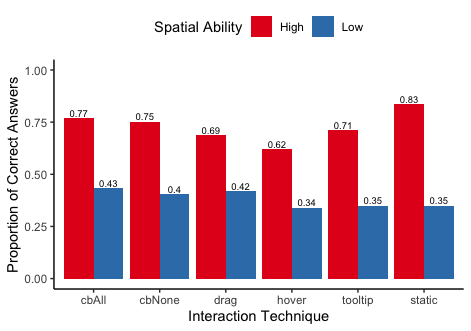
\includegraphics[width=\linewidth]{exp2_sa_by_interaction.png}
 \caption{Bar chart showing the proportion of participants answering the Bayesian reasoning task correctly by spatial ability and interaction technique. \remco{what's with the black lines above the bars? Is that a subtraction between the two bars? If so, remove please!}}
 \label{fig:exp2_sa_by_interaction}
\end{figure}

\subsubsection*{\textbf{Comparing Interaction Techniques within Spatial Ability Groups}}
Within each spatial ability group we performed a Chi-squared test of $accuracy \sim interaction\_technique$. Within the \textbf{high spatial ability} group we found a statistically significant difference in accuracy between participants using different interaction techniques ($\chi^2(5, N =  881) = 17.70, p < 0.01$). 

We performed pairwise Chi-squared tests with a Bonferroni corrected alpha ($0.003$) and found significant a pairwise difference between \textit{hover} and \textit{static} ($\chi^2(1, N = 287) = 13.60, p < 0.001$). The proportion of participants who were correct using \textit{hover} was $62\%$, whereas for the static visualization it was $83\%$ (Figure \ref{fig:exp2_sa_by_interaction}). 

Within the \textbf{low spatial ability} group we found no statistically significant difference in accuracy between participants using different interaction techniques ($\chi^2(5, N =  852) = 4.46, p = 0.49$). 

\remco{this is really cool! Would it make sense to take it one step further and look at (SA) x (interaction technique) x (base visualization)? The thought here is to see if the same message continues (that is to say, that good interactions need to be paired with good visualizations before it is useful.}
    
\subsection{Discussion} 
\remco{same comment as before... reorganize around hypotheses} Our analysis shows that interaction can narrow the performance gap between high and low spatial ability people in performing Bayesian reasoning (Figure \ref{fig:exp2_sa_by_interaction}). However it is important to note that this trend occurs in large part because \textbf{interaction decreases the performance of high spatial ability people compared to \textit{static}}. In some cases, such as with \textit{hover}, that decrease is statistically significant. On the other hand, our analyses indicate that overall \textbf{interaction increases the performance of low spatial ability people compared to \textit{static}} with the exception of \textit{hover} which produced lower accuracy than \textit{static} for both spatial ability groups.        


%\subsubsection*{H3.0}
%For every interaction technique, we found a statistically significant difference in $accuracy \sim high\_or\_low\_spatial\_ability$:
%\begin{itemize}
%	\item \textit{cbAll} ($\chi^2(1) = 25.74, p < 0.001$)
%	\item \textit{cbNone} ($\chi^2(1) = 48.23, p < 0.001$)
%	\item \textit{drag} ($\chi^2(1) = 23.14, p < 0.001$)
%	\item \textit{hover} ($\chi^2(1) = 33.94, p < 0.001$)
%	\item \textit{tooltip} ($\chi^2(1) = 52.42, p < 0.001$)
%	\item \textit{static} ($\chi^2(1) = 52.60, p < 0.001$)
%\end{itemize}

%Figure \ref{fig:accIntBaseSA} shows distributions of accuracy by each interaction technique and spatial ability and Table \ref{tab:accIntSA} shows the five number summaries plus mean and SD of accuracy for each interaction technique and spatial ability. 

%\subsubsection*{H3.1}
%Overall and within each base visualization and spatial ability group we performed  tests of $accuracy \sim interaction\_technique$. Results of each are presented below.  

%\subsubsection*{\textbf{Overall}}
%\textbf{High Spatial Ability}: Across all base visualizations we found a significant difference in accuracy between interaction techniques for people with high spatial ability ($\chi^2(5) = 21.12, p < 0.001$). A Dunn test with Bonferroni adjusted alpha showed the following significant pairwise differences:
%\begin{itemize}
%\item  \textit{cbAll} is significantly more accurate than \textit{hover} ($Z = 3.09, p-adj < 0.05$)
%\item  \textit{cbNone} is significantly more accurate than \textit{hover} ($Z = 3.09, p-adj < 0.05$)
%\item  \textit{hover} is significantly less accurate than \textit{static} ($Z = -4.02, p-adj < 0.001$)
%\end{itemize}
%Five number summaries plus mean and standard deviation are shown in Table \ref{tab:accIntSA} and Figure \ref{fig:accIntBaseSA}
 
%\noindent \textbf{Low Spatial Ability}: Across all base visualizations we found no significant difference in accuracy between interaction techniques for people with low spatial ability ($\chi^2(5) = 4.84, p = 0.44$). Five number summaries plus mean and standard deviation are shown in Table \ref{tab:accIntSA} and Figure \ref{fig:accIntBaseSA}.

%\begin{table}[h!]
%\resizebox{\linewidth}{!}{
%\centering
%\begin{tabular}{llllllll}
%  \hline
%  & Min & 1st Q & Median & 3rd Q & Max & Mean & SD \\ 
%  \hline
%cbAll - High SA & 0 & 100 & 100 & 100 & 100 & 89.5 & 21.5 \\ 
%  cbAll - Low SA & 0 & 12.5 & 62.5 & 100 & 100 & 60.3 & 41.3 \\ 
%  cbNone - High SA & 0 & 100 & 100 & 100 & 100 & 85.6 & 28.9 \\ 
%  cbNone - Low SA & 0 & 12.5 & 50 & 100 & 100 & 58.6 & 40.6 \\ 
%  drag - High SA & 0 & 75 & 100 & 100 & 100 & 81.8 & 31.1 \\ 
%  drag - Low SA & 0 & 0 & 75 & 100 & 100 & 58.9 & 42.5 \\ 
%  hover - High SA & 0 & 50 & 100 & 100 & 100 & 74.7 & 36.8 \\ 
%  hover - Low SA & 0 & 12.5 & 50 & 100 & 100 & 49.3 & 41.8 \\ 
%  tooltip - High SA & 0 & 75 & 100 & 100 & 100 & 84.2 & 28.7 \\ 
%  tooltip - Low SA & 0 & 12.5 & 50.9 & 100 & 100 & 57 & 40.3 \\ 
%  static - High SA & 0 & 100 & 100 & 100 & 100 & 90.3 & 24.6 \\ 
%  static - Low SA & 0 & 12.5 & 63.6 & 100 & 100 & 56.5 & 40.6 \\ 
 %  \hline
%\end{tabular}}
%\caption{Five number summary of accuracy for each interaction technique by high and low spatial ability (SA) across all base visualizations.  }
%\label{tab:accIntSA}
%\end{table}

%\subsubsection*{\textbf{Grouped}}
%\textbf{High Spatial Ability}: Within the grouped base visualization we found no significant difference in accuracy between interaction techniques for people with high spatial ability ($\chi^2(5) = 9.57, p = 0.09$). Five number summaries plus mean and standard deviation are shown in Table \ref{tab:accIntBaseSA} and Figure \ref{fig:accIntBaseSA}.

%\textbf{Low Spatial Ability}: Within the grouped base visualization we found no significant difference in accuracy between interaction techniques for people with low spatial ability ($\chi^2(5) = 1.69, p = 0.89$). Five number summaries plus mean and standard deviation are shown in Table \ref{tab:accIntBaseSA} and Figure \ref{fig:accIntBaseSA}.


%\subsubsection*{\textbf{Aligned}}
%\textbf{High Spatial Ability}: Within the aligned base visualization we found no significant difference in accuracy between interaction techniques for people with high spatial ability ($\chi^2(5) = 9.09, p = 0.11$). Five number summaries plus mean and standard deviation are shown in Table \ref{tab:accIntBaseSA} and Figure \ref{fig:accIntBaseSA}.

%\textbf{Low Spatial Ability}: Within the aligned base visualization we found no significant difference in accuracy between interaction techniques for people with low spatial ability ($\chi^2(5) = 8.74, p = 0.12$). Five number summaries plus mean and standard deviation are shown in Table \ref{tab:accIntBaseSA} and Figure \ref{fig:accIntBaseSA}.


%\subsubsection*{\textbf{Randomized}}
%\textbf{High Spatial Ability}: Within the randomized base visualization we found no significant difference in accuracy between interaction techniques for people with high spatial ability ($\chi^2(5) = 9.26, p = 0.10$). Five number summaries plus mean and standard deviation are shown in Table \ref{tab:accIntBaseSA} and Figure \ref{fig:accIntBaseSA}.

%\textbf{High Spatial Ability}: Within the randomized base visualization we found no significant difference in accuracy between interaction techniques for people with low spatial ability ($\chi^2(5) = 1.76, p = 0.88$). Five number summaries plus mean and standard deviation are shown in Table \ref{tab:accIntBaseSA} and Figure \ref{fig:accIntBaseSA}.

%\begin{table}[h!]
%\resizebox{\linewidth}{!}{
%\centering
%\begin{tabular}{llllllll}
%  \hline
%  & Min & 1st Q & Median & 3rd Q & Max & Mean & SD \\ 
%  \hline
%grouped - cbAll - High SA & 12.5 & 100 & 100 & 100 & 100 & 91.5 & 21.9 \\ 
%  grouped - cbAll - Low SA & 0 & 12.5 & 100 & 100 & 100 & 66.2 & 43.9 \\ 
%  grouped - cbNone - High SA & 0 & 100 & 100 & 100 & 100 & 85.8 & 28.8 \\ 
%  grouped - cbNone - Low SA & 0 & 12.5 & 62.5 & 100 & 100 & 58.8 & 42.3 \\ 
%  grouped - drag - High SA & 12.5 & 100 & 100 & 100 & 100 & 89.4 & 22 \\ 
%  grouped - drag - Low SA & 0 & 0 & 75 & 100 & 100 & 56.2 & 45.2 \\ 
%  grouped - hover - High SA & 0 & 50 & 100 & 100 & 100 & 73.7 & 37.4 \\ 
%  grouped - hover - Low SA & 0 & 0 & 50 & 100 & 100 & 53 & 44.8 \\ 
%  grouped - tooltip - High SA & 0 & 93.2 & 100 & 100 & 100 & 85.5 & 28.3 \\ 
%  grouped - tooltip - Low SA & 0 & 12.5 & 50 & 100 & 100 & 56.9 & 40.4 \\ 
%  grouped - static - High SA & 0 & 100 & 100 & 100 & 100 & 90.2 & 25.4 \\ 
%  grouped - static - Low SA & 0 & 6.3 & 75 & 100 & 100 & 56.4 & 42.3 \\ 
%  aligned - cbAll - High SA & 50 & 100 & 100 & 100 & 100 & 92.6 & 16.7 \\ 
%  aligned - cbAll - Low SA & 0 & 25 & 75 & 100 & 100 & 61.8 & 41.7 \\ 
%  aligned - cbNone - High SA & 0 & 100 & 100 & 100 & 100 & 88.5 & 24.7 \\ 
%  aligned - cbNone - Low SA & 0 & 50 & 100 & 100 & 100 & 68.6 & 37.9 \\ 
%  aligned - drag - High SA & 0 & 50 & 100 & 100 & 100 & 73.8 & 38.1 \\ 
%  aligned - drag - Low SA & 0 & 9.4 & 75 & 100 & 100 & 59.8 & 41.3 \\ 
 % aligned - hover - High SA & 0 & 75 & 100 & 100 & 100 & 80.2 & 33.6 \\ 
 % aligned - hover - Low SA & 0 & 0 & 50 & 100 & 100 & 45.1 & 40.7 \\ 
 % aligned - tooltip - High SA & 0 & 75 & 100 & 100 & 100 & 83.5 & 29.4 \\ 
%  aligned - tooltip - Low SA & 0 & 12.5 & 51.7 & 100 & 100 & 59.2 & 39.8 \\ 
%  aligned - static - High SA & 12.5 & 100 & 100 & 100 & 100 & 92.8 & 20.1 \\ 
%  aligned - static - Low SA & 0 & 40.6 & 75 & 100 & 100 & 61.3 & 39.3 \\ 
%  randomized - cbAll - High SA & 0 & 75 & 100 & 100 & 100 & 86.2 & 24 \\ 
%  randomized - cbAll - Low SA & 0 & 9.4 & 50 & 100 & 100 & 54.2 & 39.9 \\ 
%  randomized - cbNone - High SA & 0 & 75 & 100 & 100 & 100 & 82.2 & 33.1 \\ 
%  randomized - cbNone - Low SA & 0 & 12.5 & 50 & 100 & 100 & 49.6 & 39.6 \\ 
%  randomized - drag - High SA & 0 & 66.5 & 100 & 100 & 100 & 82.6 & 29.8 \\ 
%  randomized - drag - Low SA & 0 & 12.5 & 50 & 100 & 100 & 60.4 & 42.2 \\ 
%  randomized - hover - High SA & 0 & 50 & 100 & 100 & 100 & 71 & 38.7 \\ 
%  randomized - hover - Low SA & 0 & 12.5 & 50 & 100 & 100 & 49.8 & 40.6 \\ 
 % randomized - tooltip - High SA & 0 & 75 & 100 & 100 & 100 & 83.8 & 28.8 \\ 
 % randomized - tooltip - Low SA & 0 & 0 & 62.5 & 100 & 100 & 54.3 & 41.4 \\ 
%  randomized - static - High SA & 0 & 100 & 100 & 100 & 100 & 88.8 & 27 \\ 
 % randomized - static - Low SA & 0 & 3.1 & 50 & 98.7 & 100 & 49.8 & 40 \\ 
 %  \hline
%\end{tabular}}
%\caption{Five number summary of accuracy for each interaction technique by high and low spatial ability (SA) and base visualizations. }
%\label{tab:accIntBaseSA}
%\end{table}

%\begin{figure}[h!]
%\centering
%\begin{tabular}{ll}
%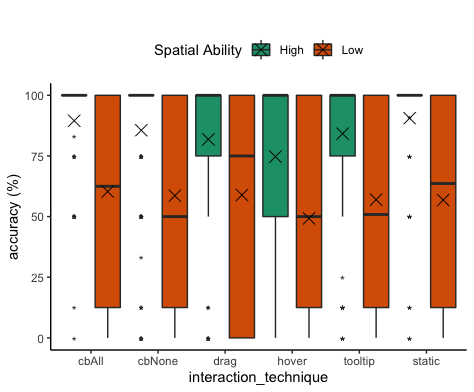
\includegraphics[height=100px]{accIntSA.png} & 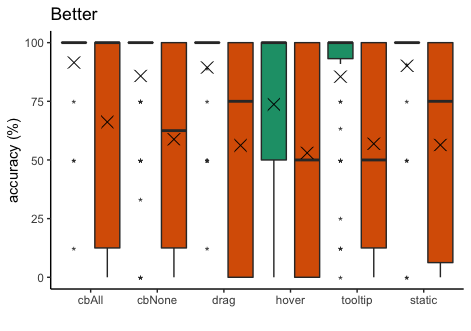
\includegraphics[height=85px]{accIntSAGrouped.png}  \\   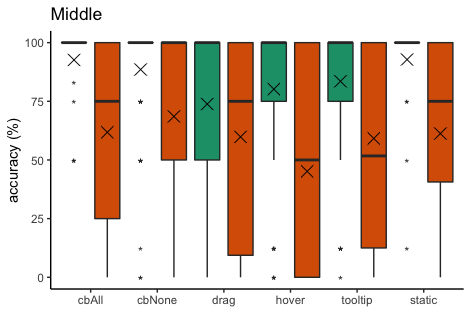
\includegraphics[height=85px]{accIntSAAligned.png} & 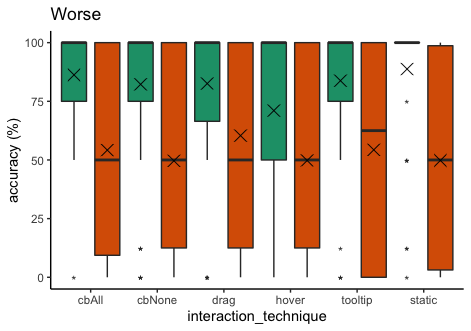
\includegraphics[height=85px]{accIntSARandomized.png} 
%\end{tabular}
% \caption{Boxplots showing the distributions of $accuracy \sim interaction\_technique * spatial\_ability$ overall (top left) and for each base visualization. X represents the mean of each distribution.}
% \label{fig:accIntBaseSA}
%\end{figure}

%\subsection{Discussion}
%Our analyses indicate that we should accept \textbf{H3.0} (there will be a significant difference in accuracy between high and low spatial ability participants for every interaction technique). No interaction techniques removed the significant difference in performance between high and low spatial ability participants.  

%Our analyses also indicate that we should accept \textbf{H3.1} (the effect of different interaction techniques on accuracy will differ between participants with high versus low spatial ability). However, not in the way we expected. Ultimately, our analyses indicated that low spatial ability participants are not significantly affected by any interaction techniques; their performance is low across the board. In contrast, we find that overall base visualizations the accuracy of high spatial ability participants could be significantly decreased by certain interaction techniques. Specifically, \textit{hover} which we found to be significantly less accurate than \textit{cbAll}, \textit{cbNone}, and even \textit{static} for high spatial ability participants.  



\section{Discussion} 
Although it is a common belief that interactivity adds value to data visualization, scientific investigations into it merits can reveal essential insights about the pros, cons, or missed opportunities in visualization design. In this experiment, we used Bayesian reasoning -- a problem that is notoriously challenging for the general population -- and showed that interactivity can in some cases detract from reasoning accuracy. 

Our analyses suggest that the value of adding interactivity depends on the design of the visualization itself. We used three variations of icon arrays based on theories for how to facilitate Bayesian reasoning: \textit{grouped}, \textit{aligned}, and \textit{randomized}. We observed nearly identical accuracy between the interactive and static versions of the \textit{grouped} and \textit{aligned} designs, and a statistically significant decrease in accuracy for the \textit{randomized} design. One rationale for this outcome is that the combination of a challenging Bayesian problem with randomness and interactivity may have induced an extraneously high cognitive load. Interactivity has been linked to increased learning in the field of multimedia learning\cite{evans2007Interactivity}, but some experts caution that adding interactivity to a significantly complicated task can result in cognitive overload\cite{mayer2001Cognitive}. Our results may be an example of this phenomenon. Due to the lack of perceptual grouping, the \textit{randomized} base visualization induces more cognitive load than the \textit{grouped} and \textit{aligned} bases and adding interaction to it may have caused cognitive overload in participants.    

Stratified analyses show this trend holds for people with high spatial ability but not for people with low spatial ability. While it is well established that spatial ability affects visualization usage~\cite{liu2020Survey} and Bayesian reasoning~\cite{ottley2016Bayesian}, our finding is surprising.
Spatial ability is typically positively correlated with effective utilization of visualization~\cite{liu2020Survey}, however our finding indicates that the opposite can be true for some interactive visualizations. We reason that this may have occurred 
because our stimuli combines text and visualization. Integrating text and visualization for Bayesian reasoning has been shown to be more difficult for people with high spatial ability than for people with low spatial ability~\cite{ottley2016Bayesian}. The \textit{cbAll} interaction attempts to create an explicit link between text labels and the visualization, thus forcing users to integrate text and visualization. It may be the case that for people with high spatial ability the high cognitive load of the \textit{randomized} base coupled with the added cognitive load of integrating text and visualization because of the \textit{cbAll} interaction results in cognitive overload. Because people with low spatial ability struggle less to integrate textual and visual representations of Bayesian inference there may be less cognitive load added by the \textit{cbAll} interaction, thus explaining why we did not observe a similar decrease in performance for this group.  

%Ottley et al.~\cite{ottley2016Bayesian} found that participants with high spatial ability performed worse on a Bayesian reasoning problem when presented with textual \textit{and} visual representations problem than when presented with one of the two. They also found this was not the case for participants with low spatial ability~\cite{ottley2016Bayesian}. 
%Interactivity has been linked to increased learning in the field of multimedia learning\cite{evans2007Interactivity}, but some experts caution that adding interactivity to a significantly complicated task can result in cognitive overload\cite{mayer2001Cognitive}. Our results may be an example of this phenomenon. Due to the lack of perceptual grouping, the randomized base visualization requires more cognitive load than the grouped and aligned bases.  
%It may be the case that for people with high spatial ability the added cognitive load of the randomized base coupled with the added cognitive load of integrating textual and visual representations of Bayesian inference (which in this study we force with interaction) results in cognitive overload. Because people with low spatial ability struggle less to integrate textual and visual representations of Bayesian inference there may be less cognitive load added by an interaction that forces such an integration, thus explaining why we did not observe a decrease in performance given interactive randomized visualization for this group.  

%do people really interact?
An important observation is that a sizable portion of our study population ($30\%$) did not use the interactive components of the visualization. There are a combination of factors that can explain this result. %First, a user can accurately solve the problem without interacting with the checkboxes. In this instance, no interaction is equivalent to the static condition \remco{I would rework these three possibilities to just focus on 2 and 3 since you immediately dismiss the first possibility right after saying that it's possible}. 
No interaction could be indicative of participants who were either confused about the task or were simply clicking through to get paid, as discussed in Section \ref{sec:exp1_analysis}. 
%Further analysis suggests that the second rationale may be more plausible. We observed that the proportion of participants in this category who answered correctly was only 40\%.
Alternatively, it is possible that participants did not want to interact. Existing work indicates that people may not engage with interactive visualizations as much as previously thought~\cite{boy2015storytelling} and there have been reports of media venues such as \textit{The New York Times}, scaling back their creation of interactive visualization in lieu of static images\footnote{\label{foot:nyt}Why We Are Doing Fewer Interactives (Archie Tse, The New York Times): https://github.com/archietse/malofiej-2016/blob/master/tse-malofiej-2016-slides.pdf}.
While understanding if there is a value-add of interaction is an important step to user-centered interactive visualization design, we recognize that understanding users' perceived value of interaction is also crucial. We leave as future work investigating users' perceived value of interaction.  %\remco{love the ending of this. It gives me chills}

\section{Design Implications} 
Our findings suggest a nuanced answer to the question ``Does interaction improve Bayesian reasoning with visualizations?'' In this section, we present a few takeaways based on the results of our experiment.

\vspace{6pt} \noindent \textbf{Design Appropriately for Context}:
Our findings suggest that the cognitive load induced by a static visualization may effect whether adding interaction will detract from its effectiveness. We found that the accuracy of participants given base visualizations that leveraged perceptual grouping to reduce cognitive load (\textit{grouped}, \textit{aligned}) was generally unaffected by the addition of interaction. In contrast, the accuracy of participants given the \textit{randomized} base visualization, which did not use any perceptual grouping to reduce cognitive load, was significantly decreased by the addition of interaction (Figure \ref{fig:exp1_static_vs_int_by_base}). This suggests that in cases where a static visualization has a high amount of cognitive load, adding interaction will likely overload users and lead to poorer performance. However, in cases where a static visualization has a minimal amount of cognitive load designers can likely add interaction without overloading users. This can be particularly useful in cases where designers wish to leverage interaction for a purpose other than improving performance, for example, improving engagement.  

\vspace{6pt} \noindent \textbf{Interactions are Not Always Necessary}: Our findings suggest that a well-designed static visualization can be as beneficial (if not better) to solving complex reasoning tasks as interactive visualizations.
%It is important to note that 
In cases where the user's interactions result in additional information being shown on the visualization (e.g. panning a map), the value of the interaction is undisputed.
However, general claims that interaction can improve reasoning, and offer cognitive support can be called into question given the results of our experiment.
We observe that in multiple cases (such as when users have high spatial ability, or the underlying visualization induces high cognitive load), the use of an interactive visualization can be detrimental. However, this study only explored one interaction design, and there are innumerable ways interaction can be added to a static visualization. Future work testing different interaction designs is needed to before making any definitive claims about the value of adding interaction to a static visualization. Based on the results of this work, we echo the sentiment made by researchers such as Lam\cite{lam2008Framework} and van Wijk\cite{wijk2005Value}, and practitioners like the New York Times, and suggest a cautious use of interactivity in visualizations.


\section{Conclusion} 
This paper aims to empirically show the how interaction may improve or detract from a static visualization. We use a classic Bayesian reasoning task as a test bed for evaluating interactive checkboxes across three different static visualization designs. Through a crowdsourced study we show the effect of interaction is largely dependent on the design of the underlying static visualization and users' spatial ability. 
Our work suggests that adding interaction to a static Bayesian reasoning visualization may not be beneficial. We find adding interactive checkboxes to a Bayesian reasoning visualization did not significantly increase performance on a Bayesian reasoning task, and some cases significantly detracted from it (for example with a cognitively taxing static visualization, particularly for users with high spatial ability). Our results point to the importance of developing good static visualizations, and weighing the cost of adding interaction against user needs and context. 







%% if specified like this the section will be committed in review mode
\acknowledgments{
This work was supported by a grant from XYZ (\# 12345-67890).
}

\bibliographystyle{abbrv}
%\bibliographystyle{abbrv-doi}
%\bibliographystyle{abbrv-doi-narrow}
%\bibliographystyle{abbrv-doi-hyperref}
%\bibliographystyle{abbrv-doi-hyperref-narrow}

\bibliography{main}
\end{document}

